% ╔══════════════════════════════════════════════════════════════════╗
% ║  PROJET 1 — FOUILLE DE DONNÉES — ENSPY 2026/2027                ║
% ║  Règles d'association FP-Growth : lac Monoun (1983–2024)         ║
% ╚══════════════════════════════════════════════════════════════════╝
% Les chiffres viennent de macros.tex et tables/ (générés par generate_assets.py).

\documentclass[12pt, a4paper]{article}

%─── Encodage & langue ────────────────────────────────────────────────
\usepackage[utf8]{inputenc}
\usepackage[T1]{fontenc}
\usepackage[french]{babel}
\usepackage{palatino}
\usepackage{microtype}
\usepackage{graphicx}
\usepackage{textcomp}

%─── Mise en page ─────────────────────────────────────────────────────
\usepackage[top=2.8cm, bottom=2.8cm, left=2.8cm, right=2.8cm, headheight=15pt]{geometry}
\usepackage{setspace}
\setstretch{1.15}
\setlength{\parskip}{4pt}
\setlength{\parindent}{1.2em}

%─── Couleurs ─────────────────────────────────────────────────────────
\usepackage[dvipsnames, table]{xcolor}
\definecolor{NuitBleue}{RGB}{10,30,65}
\definecolor{OrCam}{RGB}{188,143,20}
\definecolor{VertSav}{RGB}{0,112,60}
\definecolor{GrisP}{RGB}{248,245,238}
\definecolor{GrisL}{RGB}{240,242,246}
\definecolor{GrisB}{RGB}{180,180,190}
\definecolor{RougeL}{RGB}{180,40,40}
\definecolor{TexteP}{RGB}{25,25,35}

%─── Maths ────────────────────────────────────────────────────────────
\usepackage{amsmath,amssymb,amsthm,mathtools,bm}
\usepackage{icomma}

%─── Tableaux ─────────────────────────────────────────────────────────
\usepackage{booktabs,array,longtable,multirow,float,caption}
\captionsetup{font={small,it},labelfont={bf,color=NuitBleue},labelsep=quad,skip=5pt}
\captionsetup[table]{position=top}

%─── Boîtes ───────────────────────────────────────────────────────────
\usepackage[most]{tcolorbox}
\tcbuselibrary{skins,breakable}

\newtcolorbox{reponse}[1][Réponse]{enhanced,breakable,arc=2pt,
  colback=VertSav!5,colframe=VertSav!65!black,
  colbacktitle=VertSav!75!black,coltitle=white,
  fonttitle=\small\bfseries\scshape,
  title={\raisebox{-0.5pt}{$\triangleright$}~~#1},
  attach boxed title to top left={xshift=8pt,yshift=-\tcboxedtitleheight/2},
  boxed title style={enhanced,arc=2pt,colframe=VertSav!75!black},
  top=8pt,bottom=6pt,left=8pt,right=6pt,
  before skip=8pt,after skip=8pt}

\newtcolorbox{hypothese}[1]{enhanced,breakable,arc=2pt,
  colback=RougeL!4,colframe=RougeL!70!black,
  colbacktitle=RougeL!80!black,coltitle=white,
  fonttitle=\small\bfseries\scshape,
  title={\raisebox{-0.5pt}{$\triangleright$}~~#1},
  attach boxed title to top left={xshift=8pt,yshift=-\tcboxedtitleheight/2},
  boxed title style={enhanced,arc=2pt,colframe=RougeL!80!black},
  top=8pt,bottom=6pt,left=8pt,right=6pt,
  before skip=8pt,after skip=8pt}

\newtcolorbox{formule}[1][]{enhanced,arc=0pt,
  colback=NuitBleue!4,colframe=OrCam,
  leftrule=3.5pt,rightrule=0pt,toprule=0.4pt,bottomrule=0.4pt,
  left=10pt,right=6pt,top=5pt,bottom=5pt,
  before skip=3pt,after skip=6pt,#1}

\newtcolorbox{remarque}[1][]{enhanced,breakable,arc=2pt,
  colback=OrCam!8,colframe=OrCam!55!black,
  leftrule=3pt,rightrule=0pt,toprule=0pt,bottomrule=0pt,
  fontupper=\small\itshape,
  left=8pt,right=6pt,top=4pt,bottom=4pt,
  before skip=4pt,after skip=6pt,#1}

\newtcolorbox{code}[1][]{enhanced,arc=1pt,colback=GrisL,colframe=GrisB,
  boxrule=0.4pt,left=6pt,right=6pt,top=3pt,bottom=3pt,fontupper=\footnotesize\ttfamily,
  before skip=4pt,after skip=6pt,#1}

%─── En-têtes / pieds de page ─────────────────────────────────────────
\usepackage{fancyhdr}
\pagestyle{fancy}\fancyhf{}
\renewcommand{\headrulewidth}{0pt}
\renewcommand{\footrulewidth}{0.3pt}
\renewcommand{\footrule}{{\color{GrisB}\hrule width\headwidth height 0.3pt}}
\lhead{\color{NuitBleue}\small\scshape ENSPY · Fouille de données 2026/2027}
\rhead{\color{NuitBleue}\small\itshape Data Science — M2}
\cfoot{\color{GrisB!80!black}\small --- \thepage\ ---}
\fancypagestyle{plain}{\fancyhf{}\cfoot{\color{GrisB!80!black}\small --- \thepage\ ---}
  \renewcommand{\headrulewidth}{0pt}\renewcommand{\footrulewidth}{0.3pt}}

%─── Titres de section ────────────────────────────────────────────────
\usepackage[explicit]{titlesec}
\titleformat{\section}{\color{NuitBleue}\large\bfseries\scshape}{}
  {0pt}{\colorbox{NuitBleue!8}{\parbox{\dimexpr\linewidth-2\fboxsep}%
    {\color{NuitBleue}\large\bfseries\scshape\hspace{4pt}%
     \rule[-2pt]{3pt}{11pt}\hspace{6pt}\thesection.~#1}}}
  [\vspace{2pt}{\color{OrCam}\hrule height 0.6pt}\vspace{3pt}]
\titleformat{name=\section,numberless}{\color{NuitBleue}\large\bfseries\scshape}{}
  {0pt}{\colorbox{NuitBleue!8}{\parbox{\dimexpr\linewidth-2\fboxsep}%
    {\color{NuitBleue}\large\bfseries\scshape\hspace{4pt}%
     \rule[-2pt]{3pt}{11pt}\hspace{6pt}#1}}}
  [\vspace{2pt}{\color{OrCam}\hrule height 0.6pt}\vspace{3pt}]
\titleformat{\subsection}{\color{NuitBleue}\normalsize\bfseries}
  {\color{OrCam}\S\,\thesubsection\;}{0pt}{#1}
  [\vspace{1pt}{\color{NuitBleue!25}\hrule height 0.4pt}\vspace{2pt}]
\titleformat{\subsubsection}{\color{VertSav!80!black}\normalsize\itshape\bfseries}{}
  {0pt}{#1}
\titlespacing{\section}{0pt}{16pt}{6pt}
\titlespacing{\subsection}{0pt}{10pt}{3pt}
\titlespacing{\subsubsection}{0pt}{6pt}{2pt}

%─── Divers ───────────────────────────────────────────────────────────
\usepackage{enumitem,hyperref}
\hypersetup{colorlinks=true,linkcolor=NuitBleue,urlcolor=VertSav!70!black}
\setlist[itemize]{leftmargin=1.5em,itemsep=2pt,topsep=2pt}
\setlist[enumerate]{leftmargin=1.5em,itemsep=2pt,topsep=2pt}
\usepackage{tikz}
\usepackage{needspace}
\usetikzlibrary{positioning,arrows.meta,babel}

\newcommand{\Njours}{15\,341}
\newcommand{\Nmanquants}{0}
\newcommand{\PSaout}{88,698}
\newcommand{\PSjanv}{88,586}
\newcommand{\PSmax}{88,718}
\newcommand{\PSmaxMois}{juillet}
\newcommand{\PSmin}{88,495}
\newcommand{\PSminMois}{mars}
\newcommand{\PluieAout}{9,9}
\newcommand{\TminAout}{17,1}
\newcommand{\PnfRain}{18,3}
\newcommand{\PdixTmin}{14,9}
\newcommand{\PsoixquinzePS}{88,70}
\newcommand{\nTminWarm}{14\,558}
\newcommand{\pTminWarm}{94,9}
\newcommand{\nPressureNormal}{11\,167}
\newcommand{\pPressureNormal}{72,8}
\newcommand{\nWindCalm}{10\,178}
\newcommand{\pWindCalm}{66,3}
\newcommand{\nRainModerate}{9\,503}
\newcommand{\pRainModerate}{61,9}
\newcommand{\nDTRSuppressed}{8\,566}
\newcommand{\pDTRSuppressed}{55,8}
\newcommand{\nSeasonMonsoonPeak}{7\,098}
\newcommand{\pSeasonMonsoonPeak}{46,3}
\newcommand{\nDTRModerate}{6\,441}
\newcommand{\pDTRModerate}{42,0}
\newcommand{\nRainNone}{5\,201}
\newcommand{\pRainNone}{33,9}
\newcommand{\nWindModerate}{5\,158}
\newcommand{\pWindModerate}{33,6}
\newcommand{\nSeasonDry}{4\,463}
\newcommand{\pSeasonDry}{29,1}
\newcommand{\nSeasonTransition}{3\,780}
\newcommand{\pSeasonTransition}{24,6}
\newcommand{\nPressureHighStable}{3\,544}
\newcommand{\pPressureHighStable}{23,1}
\newcommand{\nTminCold}{767}
\newcommand{\pTminCold}{5,0}
\newcommand{\nRainExtremeDownpour}{637}
\newcommand{\pRainExtremeDownpour}{4,2}
\newcommand{\nPressureCriticalDrop}{630}
\newcommand{\pPressureCriticalDrop}{4,1}
\newcommand{\nDTRExtreme}{334}
\newcommand{\pDTRExtreme}{2,2}
\newcommand{\nTminSevereCooling}{16}
\newcommand{\pTminSevereCooling}{0,1}
\newcommand{\nWindHighShear}{5}
\newcommand{\pWindHighShear}{0,0}
\newcommand{\NreglesBrutes}{1\,572}
\newcommand{\NreglesInf}{1\,496}
\newcommand{\NreglesClean}{407}
\newcommand{\NreglesNonInf}{76}
\newcommand{\NreglesTminWarm}{279}
\newcommand{\exNX}{767}
\newcommand{\exNXY}{736}
\newcommand{\exSupp}{0,0480}
\newcommand{\exConf}{0,960}
\newcommand{\exNY}{3\,914}
\newcommand{\exSuppY}{0,255}
\newcommand{\exGain}{0,704}
\newcommand{\exLift}{3,76}
\newcommand{\pieceX}{\texttt{DTR\_Moderate}, \texttt{Pressure\_High\_Stable}, \texttt{Wind\_Moderate}}
\newcommand{\pieceConf}{0,73}
\newcommand{\pieceSuppY}{0,949}
\newcommand{\pieceGain}{$-$0,219}
\newcommand{\nrRainExtremeDownpour}{29}
\newcommand{\nrPressureCriticalDrop}{22}
\newcommand{\nrTminCold}{31}
\newcommand{\nrDTRExtreme}{16}
\newcommand{\signature}{\texttt{Pressure\_Normal}, \texttt{Rain\_Moderate}, \texttt{Season\_Monsoon\_Peak}, \texttt{Tmin\_Warm}}
\newcommand{\sigSupp}{0,233}
\newcommand{\sigMoy}{85}
\newcommand{\sigPente}{$-$10,2}
\newcommand{\sigPenteAbs}{10}
\newcommand{\sigTau}{$-$0,44}
\newcommand{\sigAvant}{94}
\newcommand{\sigApres}{60}
\newcommand{\sigMilleNeuf}{117}
\newcommand{\sigRang}{3}
\newcommand{\penteRainExtremeDownpour}{3,3}
\newcommand{\pvalRainExtremeDownpour}{0,292}
\newcommand{\pentePressureCriticalDrop}{$-$3,9}
\newcommand{\pvalPressureCriticalDrop}{0,014}
\newcommand{\penteTminCold}{$-$3,3}
\newcommand{\pvalTminCold}{0,031}
\newcommand{\penteDTRExtreme}{3,0}
\newcommand{\pvalDTRExtreme}{0,036}
\newcommand{\psAvant}{88,667}
\newcommand{\psApres}{88,703}
\newcommand{\psDelta}{0,04}
\newcommand{\rexAvant}{9,5}
\newcommand{\rexApres}{22,5}
\newcommand{\tminQuatreVingt}{16,7}
\newcommand{\tminVingt}{17,5}

\newcommand{\itm}[1]{\texttt{#1}}
% Autorise la coupure des noms d'items après les tirets bas
\AtBeginDocument{\let\oldus\_\renewcommand{\_}{\oldus\allowbreak}}
\newcommand{\tabin}[1]{\rowcolors{2}{GrisL}{white}\input{tables/#1}}

%═══════════════════════════════════════════════════════════════════════
\begin{document}
\color{TexteP}

%─── PAGE DE TITRE ────────────────────────────────────────────────────
\begin{titlepage}
\pagecolor{GrisP}
\noindent
\textcolor{VertSav}{\rule{\linewidth}{4pt}}\\[-1pt]
\textcolor{RougeL}{\rule{\linewidth}{4pt}}\\[-1pt]
\textcolor{OrCam}{\rule{\linewidth}{4pt}}

\vspace{1.6cm}
\begin{center}
\begin{tcolorbox}[enhanced,arc=0pt,colback=NuitBleue,colframe=NuitBleue,
  width=3.2cm,halign=center,left=0pt,right=0pt,top=8pt,bottom=8pt]
  \centering{\color{OrCam}\LARGE\bfseries\scshape ENSPY}
\end{tcolorbox}
\end{center}

\vspace{0.3cm}
\begin{center}
  {\large\scshape\color{NuitBleue} École Nationale Supérieure Polytechnique de Yaoundé}\\[0.2em]
  {\small\color{GrisB!80!black} B.P. 8390 — Yaoundé, Cameroun}
\end{center}

\vspace{0.9cm}
{\color{OrCam}\hrule height 0.6pt}
\vspace{0.5cm}

\begin{center}
  {\color{NuitBleue!60!black}\small\scshape Projet 1 — Fouille de données (Data Mining)}\\[0.7em]
  {\color{NuitBleue}\fontsize{17}{22}\selectfont\bfseries
    Extraction par règles d'association\\[0.2em]
    des combinaisons hydro-météorologiques extrêmes\\[0.2em]
    déclencheuses d'inversion convective au lac Monoun\\[0.5em]
    \large Analyse rétrospective de l'éruption du 15 août 1984 (1983--2024)}
\end{center}

\vspace{0.5cm}
{\color{OrCam}\hrule height 0.6pt}
\vspace{1.0cm}

\begin{center}
\begin{tabular}{r@{\hspace{8pt}:\hspace{10pt}}l}
  \scshape Filière       & Data Science (Master 2) \\[4pt]
  \scshape Année         & 2026\,/\,2027 \\[4pt]
  \scshape Mois          & Novembre 2026 \\[4pt]
  \scshape Outils        & Python (pandas), Weka 3.8 — FP-Growth \\[4pt]
  \scshape Enseignant    & \textit{[à compléter]} \\[8pt]
  \scshape Réalisé par   & FOKOUO SAADIE Luciano \\
\end{tabular}
\end{center}

\vfill
\vspace{0.7cm}
\noindent
\textcolor{OrCam}{\rule{\linewidth}{4pt}}\\[-1pt]
\textcolor{RougeL}{\rule{\linewidth}{4pt}}\\[-1pt]
\textcolor{VertSav}{\rule{\linewidth}{4pt}}
\end{titlepage}

\pagecolor{white}

%─── TABLES ───────────────────────────────────────────────────────────
\newpage
\tableofcontents
\thispagestyle{plain}
\newpage
\listoftables
\thispagestyle{plain}
\newpage
\listoffigures
\thispagestyle{plain}
\newpage

%─── GLOSSAIRE ────────────────────────────────────────────────────────
\begin{center}
  {\color{NuitBleue}\Large\bfseries\scshape Définition des mots clés}
\end{center}
\addcontentsline{toc}{section}{Définition des mots clés}
\vspace{0.3em}

\subsection*{Contexte physique}
\begin{itemize}[itemsep=3pt]
  \item \textbf{\color{NuitBleue}Éruption limnique} : Dégazage brutal d'un lac dont les eaux profondes sont sursaturées en gaz dissous (ici le CO$_2$). Le gaz libéré, plus dense que l'air, s'écoule au sol et asphyxie.
  \item \textbf{\color{NuitBleue}Stratification} : Superposition de couches d'eau de densités différentes. Tant qu'elle est stable, l'eau profonde chargée en gaz reste au fond.
  \item \textbf{\color{NuitBleue}Inversion convective} : Rupture de la stratification : l'eau de surface devient plus dense que l'eau profonde (par refroidissement, par exemple), plonge et fait remonter l'eau profonde.
  \item \textbf{\color{NuitBleue}Loi de Henry} : La quantité de gaz dissous dans un liquide est proportionnelle à la pression du gaz au-dessus du liquide : une baisse de pression diminue la solubilité du CO$_2$.
  \item \textbf{\color{NuitBleue}Réanalyse MERRA-2} : Reconstitution du climat passé par un modèle numérique qui assimile des observations. Les valeurs sont des moyennes sur une maille d'environ 50~km, pas des mesures locales.
  \item \textbf{\color{NuitBleue}NASA POWER} : Service de la NASA qui fournit des séries météorologiques journalières issues de MERRA-2 en tout point du globe.
  \item \textbf{\color{NuitBleue}DOY} : \emph{Day Of Year} : numéro du jour dans l'année (1 à 365, ou 366 les années bissextiles). Le 15 août 1984 correspond au DOY 228.
  \item \textbf{\color{NuitBleue}DTR} : \emph{Diurnal Temperature Range} : amplitude thermique du jour, $T_{\max} - T_{\min}$. Faible sous un ciel couvert, forte par temps sec et dégagé.
  \item \textbf{\color{NuitBleue}Centile ($P_{10}$, $P_{95}$)} : Valeur sous laquelle se trouvent 10~\% (respectivement 95~\%) des observations.
\end{itemize}

\subsection*{Fouille de données}
\begin{itemize}[itemsep=3pt]
  \item \textbf{\color{NuitBleue}Discrétisation} : Transformation d'une variable numérique en classes (« pluie modérée », « pluie extrême »…) à l'aide de seuils.
  \item \textbf{\color{NuitBleue}Item} : Modalité binaire, présente ou absente un jour donné (ex. \itm{Rain\_Extreme\_Downpour}).
  \item \textbf{\color{NuitBleue}Transaction} : Ensemble des items observés pour une unité. Ici, une transaction est \textbf{un jour}, qui contient exactement 6 items.
  \item \textbf{\color{NuitBleue}Motif (itemset)} : Sous-ensemble non vide d'items. Un motif de $k$ items est un $k$-motif.
  \item \textbf{\color{NuitBleue}Règle d'association} : Implication $X \rightarrow Y$ entre deux motifs disjoints : $X$ est la \textbf{prémisse}, $Y$ le \textbf{conséquent}.
  \item \textbf{\color{NuitBleue}Support} : Proportion des transactions qui contiennent un motif (ou la prémisse et le conséquent d'une règle). Mesure la \emph{fréquence}.
  \item \textbf{\color{NuitBleue}Confiance} : Proportion des transactions contenant $X$ qui contiennent aussi $Y$ ; estimation de $P(Y \mid X)$. Mesure la \emph{fiabilité} de la règle.
  \item \textbf{\color{NuitBleue}minSupp, minConf} : Seuils minimaux de support et de confiance fixés par l'utilisateur.
  \item \textbf{\color{NuitBleue}Anti-monotonie} : Si $M_1 \subseteq M_2$, alors $\operatorname{supp}(M_1) \geq \operatorname{supp}(M_2)$ : ajouter des items ne peut que faire baisser le support.
  \item \textbf{\color{NuitBleue}Apriori} : Algorithme du cours, de type « générer-et-élaguer » : il génère les motifs candidats de taille $k+1$ à partir des motifs fréquents de taille $k$.
  \item \textbf{\color{NuitBleue}FP-Growth} : Algorithme de type « diviser-pour-régner » (Han et al., 2000) : il compresse la base dans un arbre (FP-tree) et extrait les motifs fréquents sans générer de candidats. Même résultat qu'Apriori.
  \item \textbf{\color{NuitBleue}Weka} : Logiciel de fouille de données de l'université de Waikato, utilisé en cours.
  \item \textbf{\color{NuitBleue}ARFF} : \emph{Attribute-Relation File Format} : format de fichier texte natif de Weka.
  \item \textbf{\color{NuitBleue}Règle informative} : Règle telle que $\operatorname{conf}(X \rightarrow Y) > \operatorname{supp}(Y)$ : connaître $X$ rend $Y$ plus fréquent qu'en moyenne.
  \item \textbf{\color{NuitBleue}Écart} : $\operatorname{conf}(X \rightarrow Y) - \operatorname{supp}(Y)$ : gain de fréquence de $Y$ apporté par $X$. Le rapport correspondant est appelé \emph{lift}.
  \item \textbf{\color{NuitBleue}Règle redondante} : Règle $X \rightarrow Y$ pour laquelle une prémisse plus courte $X' \subset X$ donne une confiance au moins égale.
\end{itemize}

\subsection*{Analyse temporelle}
\begin{itemize}[itemsep=3pt]
  \item \textbf{\color{NuitBleue}Fenêtre pré-éruption} : Les 7 jours qui précèdent l'éruption, jour de l'éruption inclus (DOY 222 à 228 de 1984).
  \item \textbf{\color{NuitBleue}Signature} : Motif présent tous les jours de la fenêtre pré-éruption.
  \item \textbf{\color{NuitBleue}Test de Mann-Kendall} : Test non paramétrique de tendance monotone d'une série temporelle. Il repose sur le $\tau$ de Kendall entre le temps et la série.
  \item \textbf{\color{NuitBleue}p-valeur} : Probabilité d'observer une tendance au moins aussi marquée si la série n'avait en réalité aucune tendance. En dessous de 0,05, la tendance est jugée significative.
\end{itemize}
\newpage

\needspace{12\baselineskip}
%═══════════════════════════════════════════════════════════════════════
\section{Introduction}
%═══════════════════════════════════════════════════════════════════════

\subsection{Contexte}

Le lac Monoun est un lac de cratère de l'Ouest du Cameroun. Ses eaux profondes, privées
d'oxygène, accumulent depuis des millénaires du CO$_2$ d'origine magmatique. Dans la nuit du
15 au 16 août 1984, ce gaz s'est brusquement dégagé : le nuage de CO$_2$ a tué
\textbf{37 personnes} par asphyxie (Sigurdsson et al., 1987). Deux ans plus tard, un
événement semblable au lac Nyos faisait plus de 1\,700 victimes.

Une éruption limnique suppose que la stratification du lac soit rompue : les eaux profondes,
chargées en gaz, remontent vers la surface où la pression chute, et le gaz sort de solution
comme d'une bouteille de boisson gazeuse que l'on ouvre. La question est alors : \emph{qu'est-ce
qui a rompu la stratification le 15 août 1984 ?}

\subsection{Problème posé}

L'énoncé du projet propose une piste \textbf{météorologique}. Certaines conditions météo
pourraient, en se combinant, déstabiliser le lac :
\begin{itemize}
  \item une \textbf{chute de pression atmosphérique}, qui abaisse la solubilité du CO$_2$
        (loi de Henry) ;
  \item un \textbf{refroidissement de surface} (nuits froides, pluies froides) qui rend l'eau
        de surface plus dense et la fait plonger (inversion convective) ;
  \item des \textbf{pluies torrentielles} et un \textbf{vent fort}, qui brassent et
        déstabilisent la couche de surface.
\end{itemize}

Le projet consiste à appliquer l'algorithme \textbf{FP-Growth} sur 42 ans de données
météorologiques journalières (1983--2024) pour :
\begin{enumerate}
  \item découvrir les \textbf{règles d'association} qui relient ces conditions météo ;
  \item identifier la \textbf{« signature de risque »} qui a précédé la catastrophe de 1984 ;
  \item mesurer la \textbf{fréquence de réapparition} de cette signature jusqu'en 2024, dans le
        contexte du réchauffement climatique.
\end{enumerate}

\subsection{Organisation du document}

La section~\ref{sec:hypotheses} traduit le problème en hypothèses testables. La
section~\ref{sec:metriques} définit les métriques et ce que chacune permet de conclure. La
section~\ref{sec:demarche} décrit le processus de travail, du fichier brut aux règles. La
section~\ref{sec:resultats} présente et interprète les résultats. La
section~\ref{sec:verdict} confronte chaque hypothèse aux résultats, avant la discussion et la
conclusion.

\needspace{12\baselineskip}
%═══════════════════════════════════════════════════════════════════════
\section{Problématique et hypothèses}
\label{sec:hypotheses}
%═══════════════════════════════════════════════════════════════════════

\begin{formule}
\textbf{Question centrale.} Les jours qui ont précédé l'éruption du lac Monoun présentent-ils
une combinaison de conditions météorologiques extrêmes, et cette combinaison devient-elle plus
fréquente avec le temps ?
\end{formule}

Pour y répondre avec des règles d'association, nous avons décomposé la question en quatre
hypothèses. Chacune est formulée de façon à pouvoir être \textbf{validée ou rejetée} par une
mesure précise.

\begin{hypothese}{H0 — Hypothèse méthodologique : des seuils climatologiques}
Les seuils de discrétisation de l'énoncé correspondent aux centiles climatologiques qu'il
annonce (« $P_{10}$, $P_{75}$, $P_{90}$, $P_{95}$ sont les centiles climatologiques »). Par
exemple, \itm{Tmin\_Severe\_Cooling} ($< 11$ °C) correspond au $P_{10}$ de la température
minimale et \itm{Rain\_Extreme\_Downpour} ($> 20$ mm) au $P_{95}$ de la pluie.

\textbf{Test :} calculer les centiles réels de la série et la part de jours de chaque item.
\end{hypothese}

\begin{hypothese}{H1 — Les extrêmes se combinent en événements composites}
Les conditions extrêmes (chute de pression, refroidissement, pluie torrentielle, vent fort)
surviennent ensemble : il existe des règles d'association fréquentes et fiables qui les
relient entre elles.

\textbf{Test :} chercher, parmi les règles extraites, celles qui contiennent au moins deux items
extrêmes ; compter les jours où ces items coïncident ; regarder à quelles conditions chaque item
extrême est associé.
\end{hypothese}

\begin{hypothese}{H2 — Une signature extrême a précédé l'éruption}
Les jours qui précèdent le 15 août 1984 présentent une combinaison de conditions extrêmes
(la « signature de risque »), inhabituelle par rapport au reste de la série.

\textbf{Test :} décrire les items des 7 jours précédant l'éruption, en extraire le motif commun
(la signature), mesurer son support et la place de 1984 parmi les autres années ; vérifier la
robustesse avec des fenêtres de 3, 14 et 30 jours.
\end{hypothese}

\begin{hypothese}{H3 — La signature réapparaît de plus en plus avec le réchauffement}
La signature pré-éruption, et plus largement les conditions extrêmes, deviennent plus
fréquentes entre 1983 et 2024.

\textbf{Test :} compter chaque année les jours qui présentent la signature et chaque item
extrême ; estimer la pente (jours par décennie) et tester la tendance (Mann-Kendall, seuil
5~\%).
\end{hypothese}

\begin{table}[H]
\centering
\caption{Correspondance entre hypothèses, tests, métriques et sections du rapport.}
\label{tab:plan_hyp}
\small
\rowcolors{2}{GrisL}{white}
\begin{tabular}{p{1.1cm}>{\raggedright\arraybackslash}p{5.4cm}>{\raggedright\arraybackslash}p{4.6cm}p{2.2cm}}
\toprule
\rowcolor{NuitBleue!90}
\color{white}\textbf{Hyp.} & \color{white}\textbf{Ce qu'il faut observer pour la valider} & \color{white}\textbf{Métriques} & \color{white}\textbf{Sections} \\
\midrule
H0 & Centiles réels proches des seuils ; items extrêmes autour de 5 à 10~\% des jours & Centiles, part des items & \ref{sec:eda}, \ref{sec:discretisation} \\
H1 & Règles reliant plusieurs items extrêmes ; jours composites nombreux & Support, confiance, écart, comptages & \ref{sec:res_extremes}, \ref{sec:res_composites} \\
H2 & Items extrêmes dans la fenêtre ; signature rare et 1984 exceptionnel & Support de la signature, rang de 1984 & \ref{sec:res_fenetre} \\
H3 & Pente positive et significative & Jours/an, pente, $\tau$, p-valeur & \ref{sec:res_temps} \\
\bottomrule
\end{tabular}
\end{table}

\needspace{12\baselineskip}
%═══════════════════════════════════════════════════════════════════════
\section{Métriques utilisées et ce qu'elles disent}
\label{sec:metriques}
%═══════════════════════════════════════════════════════════════════════

\subsection{Les métriques de base du cours : support et confiance}

Soit $n$ le nombre total de transactions (ici $n = \Njours$ jours), $n(M)$ le nombre de
transactions qui contiennent tous les items du motif $M$, et une règle $R : X \rightarrow Y$.

\begin{formule}
\[
\operatorname{supp}(M) = \frac{n(M)}{n}
\qquad
\operatorname{supp}(X \rightarrow Y) = \operatorname{supp}(X \cup Y)
\]
\[
\operatorname{conf}(X \rightarrow Y) = \frac{\operatorname{supp}(X \cup Y)}{\operatorname{supp}(X)}
\]
\end{formule}

\begin{itemize}
  \item \textbf{Le support mesure la fréquence de la règle.} C'est la part des jours où la
        règle s'observe en entier. Un support faible signifie que la règle repose sur peu de jours :
        elle peut être un hasard. Le seuil \textbf{minSupp} écarte ces règles trop rares.
  \item \textbf{La confiance mesure la fiabilité de la règle.} C'est la probabilité
        conditionnelle $P(Y \mid X)$ : parmi les jours qui présentent $X$, la part qui présente
        aussi $Y$. Le seuil \textbf{minConf} écarte les règles peu fiables.
\end{itemize}

\begin{reponse}[Exemple de calcul sur nos données]
Règle $\{\itm{Tmin\_Cold}\} \rightarrow \{\itm{Rain\_None}, \itm{Season\_Dry}\}$, extraite
par Weka :
\begin{itemize}
  \item $n(X) = \exNX$ jours de nuit froide ; $n(X \cup Y) = \exNXY$ de ces jours sont aussi
        secs et en saison sèche ;
  \item $\operatorname{supp} = \exNXY / \Njours = \exSupp$ : la règle s'observe sur 4,8~\% des
        jours ;
  \item $\operatorname{conf} = \exNXY / \exNX = \exConf$ : \textbf{96~\% des nuits froides
        tombent un jour sec de saison sèche}.
\end{itemize}
\end{reponse}

\subsection{La limite de la confiance}

La confiance seule peut tromper. Elle ne tient pas compte de la fréquence \emph{habituelle} du
conséquent. L'item \itm{Tmin\_Warm} est présent \pTminWarm~\% des jours : n'importe quelle
règle $X \rightarrow \{\itm{Tmin\_Warm}\}$ obtient donc une confiance proche de 0,95, quelle que
soit la prémisse, simplement parce que les nuits douces sont presque toujours là.

\begin{remarque}
Exemple réel : la règle $\{\pieceX\} \rightarrow \{\itm{Tmin\_Warm}\}$ a une confiance de
\pieceConf, au-dessus de minConf = 0,7. Elle semble donc « valide ». Pourtant
$\operatorname{supp}(\itm{Tmin\_Warm}) = \pieceSuppY$ : ces conditions rendent en réalité les
nuits douces \emph{moins} fréquentes que d'habitude. La confiance élevée cache une association
négative.
\end{remarque}

\subsection{La métrique que nous avons regardée : l'écart à la fréquence habituelle}

Pour corriger ce biais tout en restant dans le cadre du cours, nous comparons deux quantités
qu'il définit : la confiance de la règle et le support du conséquent.

\begin{formule}
\[
\text{écart}(X \rightarrow Y) = \operatorname{conf}(X \rightarrow Y) - \operatorname{supp}(Y)
\]
\[
\text{règle informative} \iff \operatorname{conf}(X \rightarrow Y) > \operatorname{supp}(Y)
\iff \text{écart} > 0
\]
\end{formule}

\begin{itemize}
  \item \textbf{Ce qu'il dit :} de combien la présence de $X$ augmente la probabilité de $Y$ par
        rapport à un jour quelconque. Un écart positif signale une association réelle ; un écart
        nul ou négatif, une règle sans intérêt ou trompeuse.
  \item \textbf{Pourquoi celui-ci :} il se calcule uniquement avec le support et la confiance
        du cours, et il neutralise les items omniprésents comme \itm{Tmin\_Warm}. Le cours
        prévoit d'ailleurs explicitement « le support et la confiance (ou tout autre critère de
        qualité choisi) ».
  \item \textbf{Lien avec la littérature :} le rapport
        $\operatorname{conf}(X \rightarrow Y) / \operatorname{supp}(Y)$ est la mesure appelée
        \emph{lift}. Nous utilisons la différence plutôt que le rapport pour rester sur les
        notions du cours, mais les deux classent les règles dans le même sens pour un
        conséquent donné.
\end{itemize}

Sur l'exemple précédent : $\operatorname{supp}(\{\itm{Rain\_None}, \itm{Season\_Dry}\}) =
\exNY / \Njours = \exSuppY$. L'écart vaut $\exConf - \exSuppY = \exGain$ (lift $= \exLift$) :
une nuit froide multiplie par près de 4 la probabilité d'être un jour sec de saison sèche.

Nous avons aussi retiré les \textbf{règles redondantes} : $X \rightarrow Y$ est retirée s'il
existe $X' \subset X$ tel que $X' \rightarrow Y$ ait une confiance au moins égale. Ajouter un
item à la prémisse sans gagner en fiabilité n'apporte rien.

\subsection{Les métriques de l'analyse temporelle}

\begin{itemize}
  \item \textbf{Jours par an} présentant un motif : mesure directe de sa fréquence de
        réapparition.
  \item \textbf{Pente} d'une régression linéaire du nombre de jours sur l'année, exprimée en
        jours par décennie : ampleur de la tendance.
  \item \textbf{Test de Mann-Kendall} ($\tau$ de Kendall et p-valeur) : la tendance est jugée
        significative si $p < 0{,}05$. Ce test ne suppose pas de distribution normale, ce qui
        convient à des comptages annuels.
\end{itemize}

\needspace{12\baselineskip}
%═══════════════════════════════════════════════════════════════════════
\section{Démarche : du fichier brut aux règles}
\label{sec:demarche}
%═══════════════════════════════════════════════════════════════════════

La figure~\ref{fig:pipeline} résume le processus. Le code est organisé en fonctions Python
(\texttt{src/}) appelées depuis deux notebooks, et l'extraction des règles est faite dans Weka.

\begin{figure}[H]
\centering
\setlength{\parindent}{0pt}
\begin{tikzpicture}[
  box/.style={draw=NuitBleue!70, fill=white, rounded corners=3pt, align=center,
              font=\footnotesize, minimum width=2.8cm, text width=2.65cm,
              minimum height=1.45cm, inner sep=2pt},
  weka/.style={box, draw=OrCam!90!black, fill=OrCam!10, minimum width=3.6cm, text width=3.4cm},
  res/.style={box, draw=VertSav!80!black, fill=VertSav!8},
  lanelabel/.style={font=\scriptsize\bfseries\scshape, text=NuitBleue, rotate=90},
  arr/.style={-{Stealth[length=2.2mm]}, NuitBleue!75, line width=0.8pt}]
  % bandes
  \fill[NuitBleue!5, rounded corners=4pt] (-1.7, 1.0) rectangle (13.45, -1.0);
  \fill[OrCam!7, rounded corners=4pt]     (-1.7,-1.4) rectangle (13.45, -3.4);
  \fill[VertSav!6, rounded corners=4pt]   (-1.7,-3.8) rectangle (13.45, -5.8);
  \node[lanelabel] at (-1.4, 0)   {Préparation};
  \node[lanelabel] at (-1.4,-2.4) {Extraction};
  \node[lanelabel] at (-1.4,-4.8) {Analyse};
  % phase 1 : Python
  \node[box] (a) at (0.35,0)     {\textbf{Données}\\NASA POWER\\1983--2024};
  \node[box] (b) at (3.3,0)   {\textbf{Nettoyage}\\en-tête, $-999$\\calcul du DTR};
  \node[box] (c) at (6.25,0)   {\textbf{Exploration}\\saisons\\distributions};
  \node[box] (d) at (9.2,0)   {\textbf{Discrétisation}\\18 items\\6 par jour};
  \node[box] (e) at (12.15,0)  {\textbf{Encodage}\\binaire \{0, 1\}\\fichier ARFF};
  % phase 2 : Weka
  \node[weka] (f) at (6.25,-2.4) {\textbf{FP-Growth (Weka)}\\3 essais, minSupp :\\0,10 ; 0,05 ; 0,01};
  % phase 3 : Python
  \node[box] (g) at (1.8,-4.8)  {\textbf{Filtrage}\\conf $>$ supp($Y$)\\sans redondance};
  \node[box] (h) at (4.75,-4.8)  {\textbf{Fenêtre 1984}\\signature\\pré-éruption};
  \node[box] (i) at (7.7,-4.8)  {\textbf{Réapparition}\\jours par an\\tendances};
  \node[res] (j) at (10.65,-4.8) {\textbf{Verdict}\\hypothèses\\H0 à H3};
  % flèches
  \draw[arr] (a) -- (b); \draw[arr] (b) -- (c); \draw[arr] (c) -- (d); \draw[arr] (d) -- (e);
  \draw[arr] (e.south) |- (f.east);
  \draw[arr] (f.west) -| (g.north);
  \draw[arr] (g) -- (h); \draw[arr] (h) -- (i); \draw[arr] (i) -- (j);
\end{tikzpicture}
\caption{Processus de travail en trois phases : préparation des données en Python
(\texttt{01\_preparation.ipynb}), extraction des règles dans Weka, puis analyse en Python
(\texttt{02\_analyse.ipynb}).}
\label{fig:pipeline}
\end{figure}

\subsection{Acquisition et nettoyage}
\label{sec:nettoyage}

Les données viennent de NASA POWER (réanalyse MERRA-2) au point 5,58° N -- 10,586° E, à
1\,151~m d'altitude (moyenne de la maille), du 1\textsuperscript{er} janvier 1983 au 31
décembre 2024. Le nettoyage a consisté à :
\begin{enumerate}
  \item \textbf{retirer l'en-tête descriptif} du fichier NASA, repéré par la ligne
        \texttt{-END HEADER-} plutôt que par un nombre de lignes codé en dur ;
  \item \textbf{contrôler les valeurs manquantes}, que NASA POWER code $-999$ :
        \Nmanquants~valeur manquante sur \Njours~jours, aucune imputation n'a donc été
        nécessaire ;
  \item \textbf{calculer l'amplitude thermique} $\text{DTR} = T_{\max} - T_{\min}$, arrondie à
        2 décimales comme les données sources, pour éviter qu'une valeur comme 8,000000001
        sorte artificiellement de sa classe.
\end{enumerate}

\begin{table}[H]
\centering
\caption{Variables utilisées et statistiques descriptives (1983--2024).}
\label{tab:descriptives}
\tabin{tab_descriptives}
\end{table}

\subsection{Analyse exploratoire du jeu de données}
\label{sec:eda}

\paragraph{Cycle saisonnier.} La figure~\ref{fig:climatologie} montre les moyennes mensuelles.
Août, le mois de l'éruption, est le cœur de la mousson : c'est le mois le plus pluvieux
(\PluieAout~mm/j en moyenne), avec une faible amplitude thermique (ciel couvert) et des nuits
douces (\TminAout~°C). La pression suit un cycle marqué : elle est la plus basse en
\PSminMois{} (\PSmin~kPa) et la plus haute en \PSmaxMois{} (\PSmax~kPa). En août, elle vaut en
moyenne \PSaout~kPa, \textbf{presque exactement le seuil de 88,7~kPa} qui sépare
\itm{Pressure\_Normal} de \itm{Pressure\_High\_Stable}.

\begin{figure}[H]
\centering
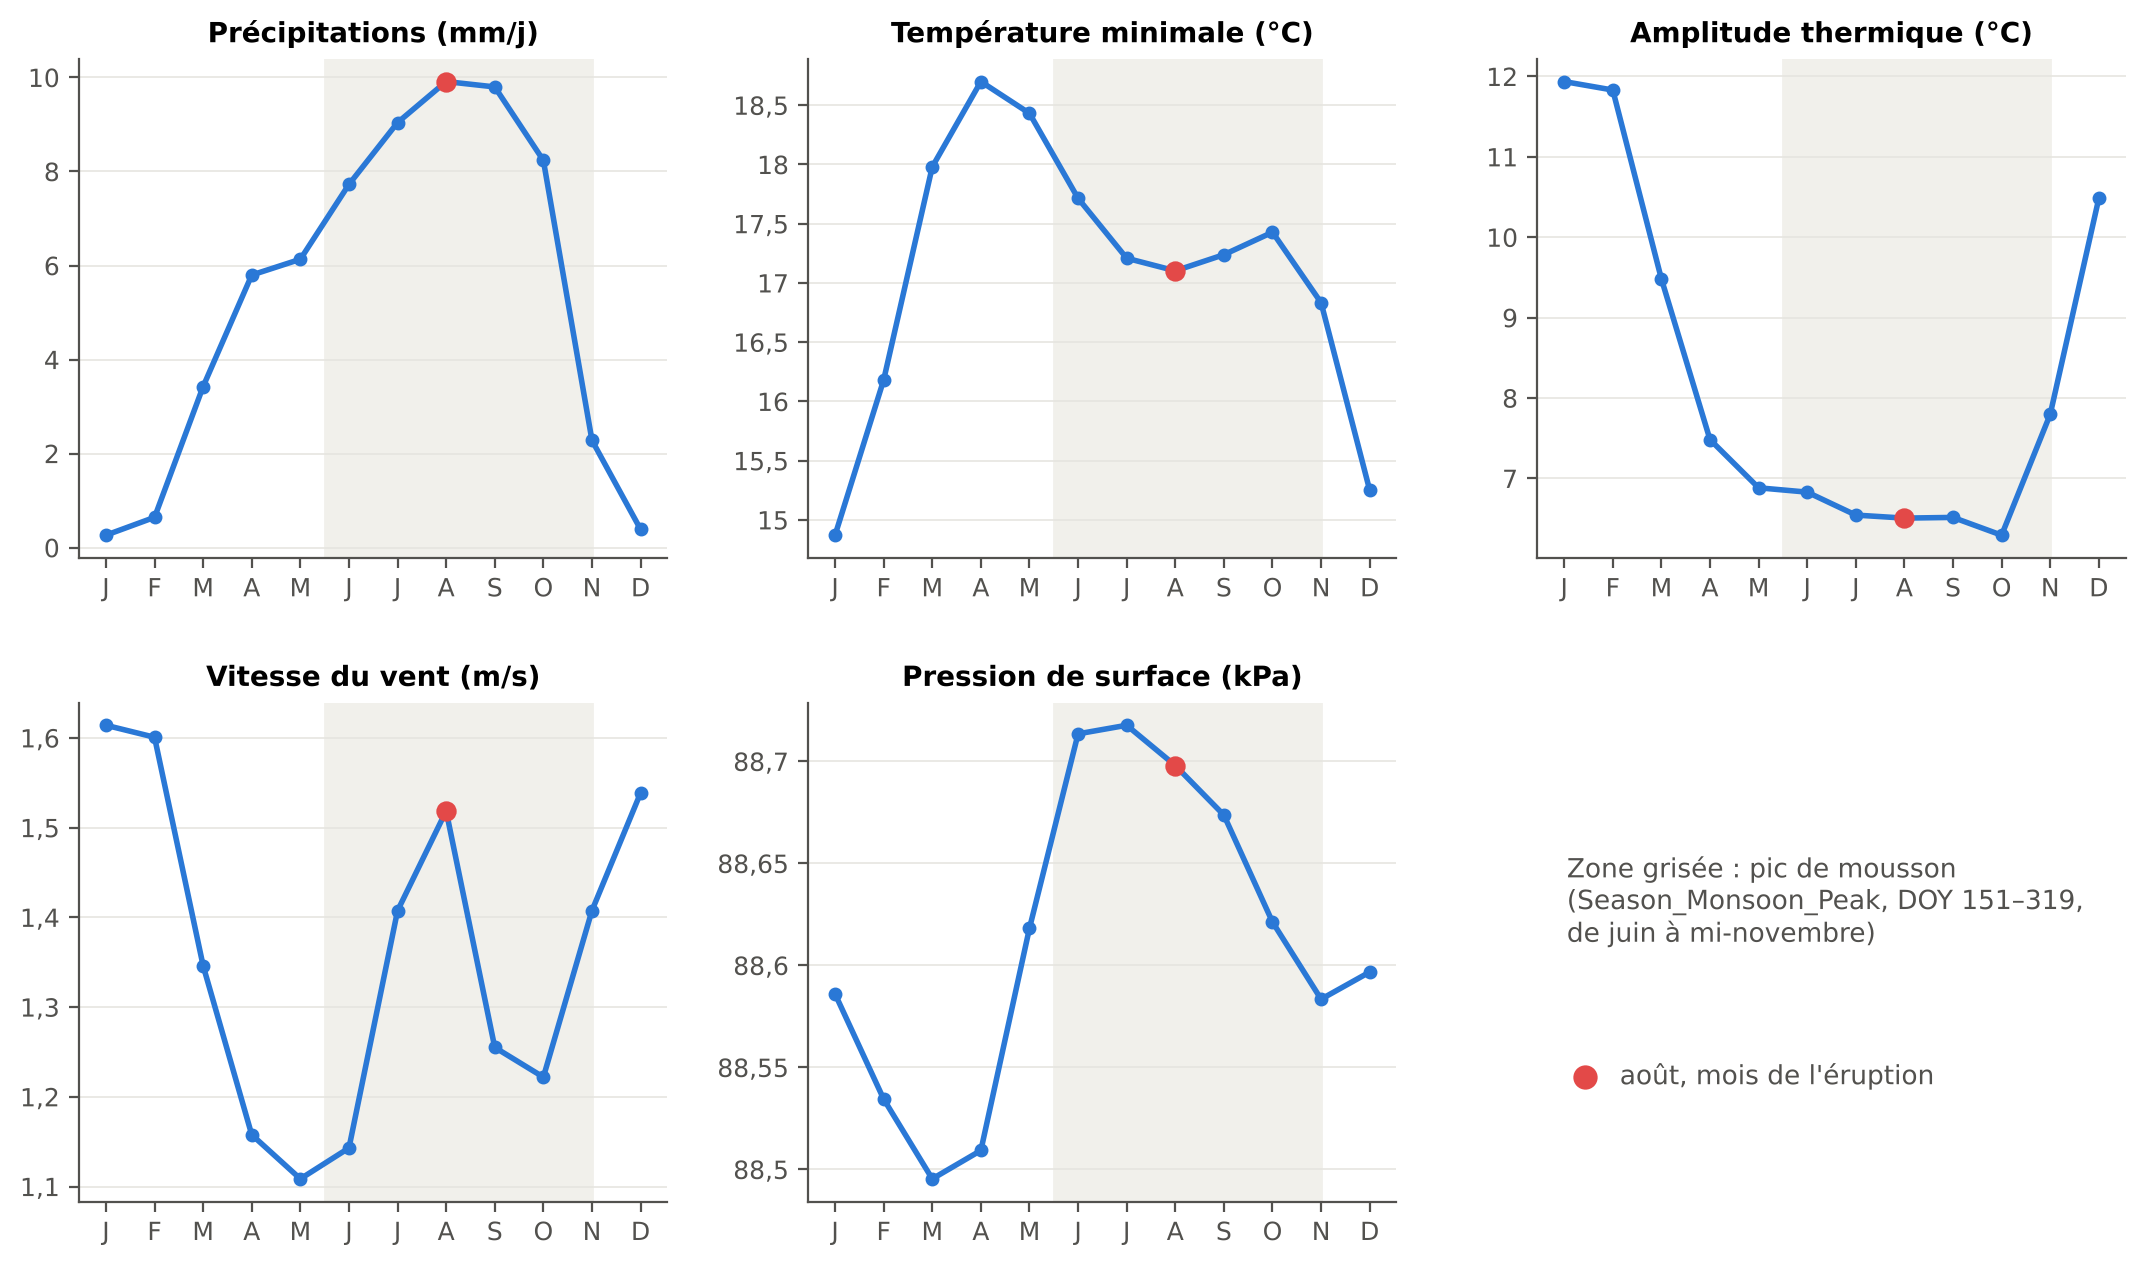
\includegraphics[width=\linewidth]{figures/fig_climatologie}
\caption{Moyennes mensuelles des variables (1983--2024).}
\label{fig:climatologie}
\end{figure}

\paragraph{Distributions et seuils.} La figure~\ref{fig:histogrammes} superpose les seuils de
l'énoncé aux distributions. Deux seuils tombent dans des zones presque vides : très peu de
jours ont une température minimale inférieure à 11~°C ou un vent supérieur à 3~m/s.

\begin{figure}[H]
\centering
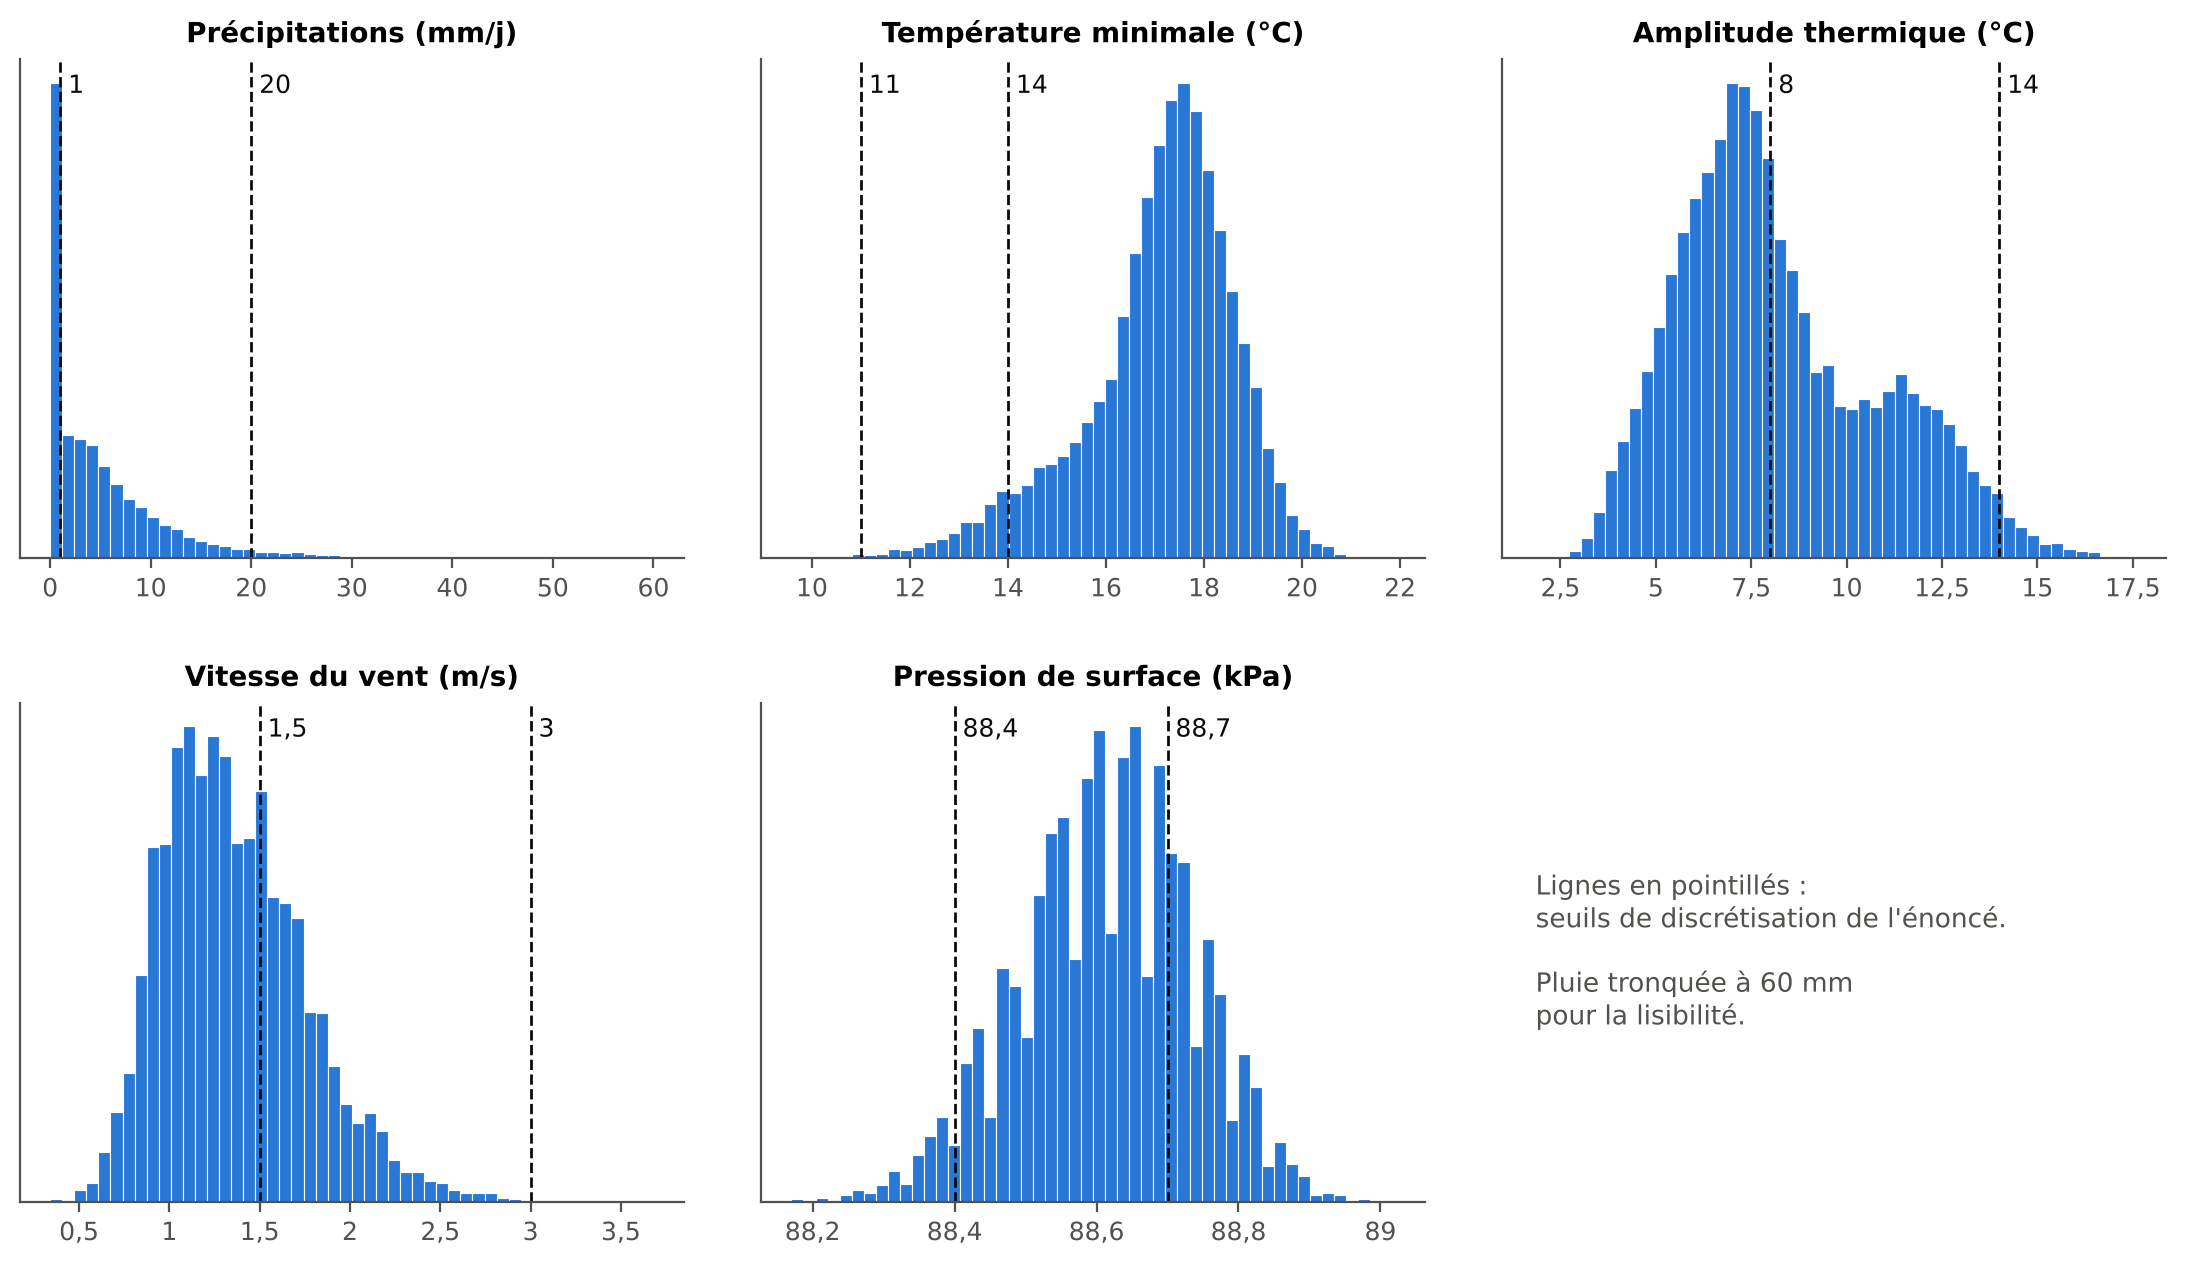
\includegraphics[width=\linewidth]{figures/fig_histogrammes}
\caption{Distributions des variables et seuils de discrétisation de l'énoncé.}
\label{fig:histogrammes}
\end{figure}

\paragraph{Test de l'hypothèse H0.} Le tableau~\ref{tab:centiles} compare les seuils aux
centiles annoncés. Le seuil de pluie extrême est cohérent avec le $P_{95}$ réel
(\PnfRain~mm). En revanche, le $P_{10}$ réel de la température minimale est de
\PdixTmin~°C, et non de 11~°C : l'item \itm{Tmin\_Severe\_Cooling} ne couvre que
\nTminSevereCooling~jours (\pTminSevereCooling~\%) au lieu des 10~\% attendus.

\begin{table}[H]
\centering
\caption{Seuils de l'énoncé et centiles réels de la série.}
\label{tab:centiles}
\tabin{tab_centiles}
\end{table}

\paragraph{Valeurs égales aux seuils.} Les données ont 2 décimales, si bien que de nombreux jours
tombent exactement sur un seuil (tableau~\ref{tab:egalites}). Pour le vent et la pression, ce
sont plusieurs centaines de jours : la règle d'affectation des bornes n'est pas un détail.

\begin{table}[H]
\centering
\caption{Nombre de jours dont la valeur est exactement égale à un seuil.}
\label{tab:egalites}
\tabin{tab_egalites}
\end{table}

\subsection{Discrétisation}
\label{sec:discretisation}

Les règles d'association classiques portent sur des données binaires. Chaque variable a donc
été découpée en trois classes selon les seuils de l'énoncé, \textbf{utilisés tels quels} pour
respecter la consigne. Trois choix ont dû être faits et justifiés :

\begin{enumerate}
  \item \textbf{Bornes.} L'énoncé définit toujours les classes extrêmes par des inégalités
        strictes ($< 1$ mm, $> 20$ mm, $> 14$ °C, $< 88{,}4$ kPa…). Une valeur égale à un seuil
        ne peut donc pas appartenir à une classe extrême : elle est affectée à la
        \textbf{classe intermédiaire}, qui forme un intervalle fermé. Pour la pluie, ce choix
        rejoint la convention internationale ETCCDI, selon laquelle un jour est pluvieux à
        partir de 1~mm. Seul écart : l'ETCCDI compte 20~mm comme « très fortes pluies »
        (indice R20mm, $\geq 20$ mm) ; nous suivons l'énoncé, ce qui ne concerne que 2 jours.
  \item \textbf{Saison sèche.} Elle chevauche le changement d'année (DOY 320 à 060) et est
        codée par la condition « DOY $\geq 320$ ou DOY $\leq 60$ ».
  \item \textbf{Années bissextiles.} Le décalage d'un jour des limites de saison après le
        29 février est négligé.
\end{enumerate}

Chaque jour devient ainsi une \textbf{transaction de 6 items} parmi 18 possibles
(tableau~\ref{tab:items} et figure~\ref{fig:items}).

\begin{table}[H]
\centering
\caption{Discrétisation : items, conditions et répartition sur 1983--2024.}
\label{tab:items}
\tabin{tab_items}
\end{table}

\begin{figure}[H]
\centering
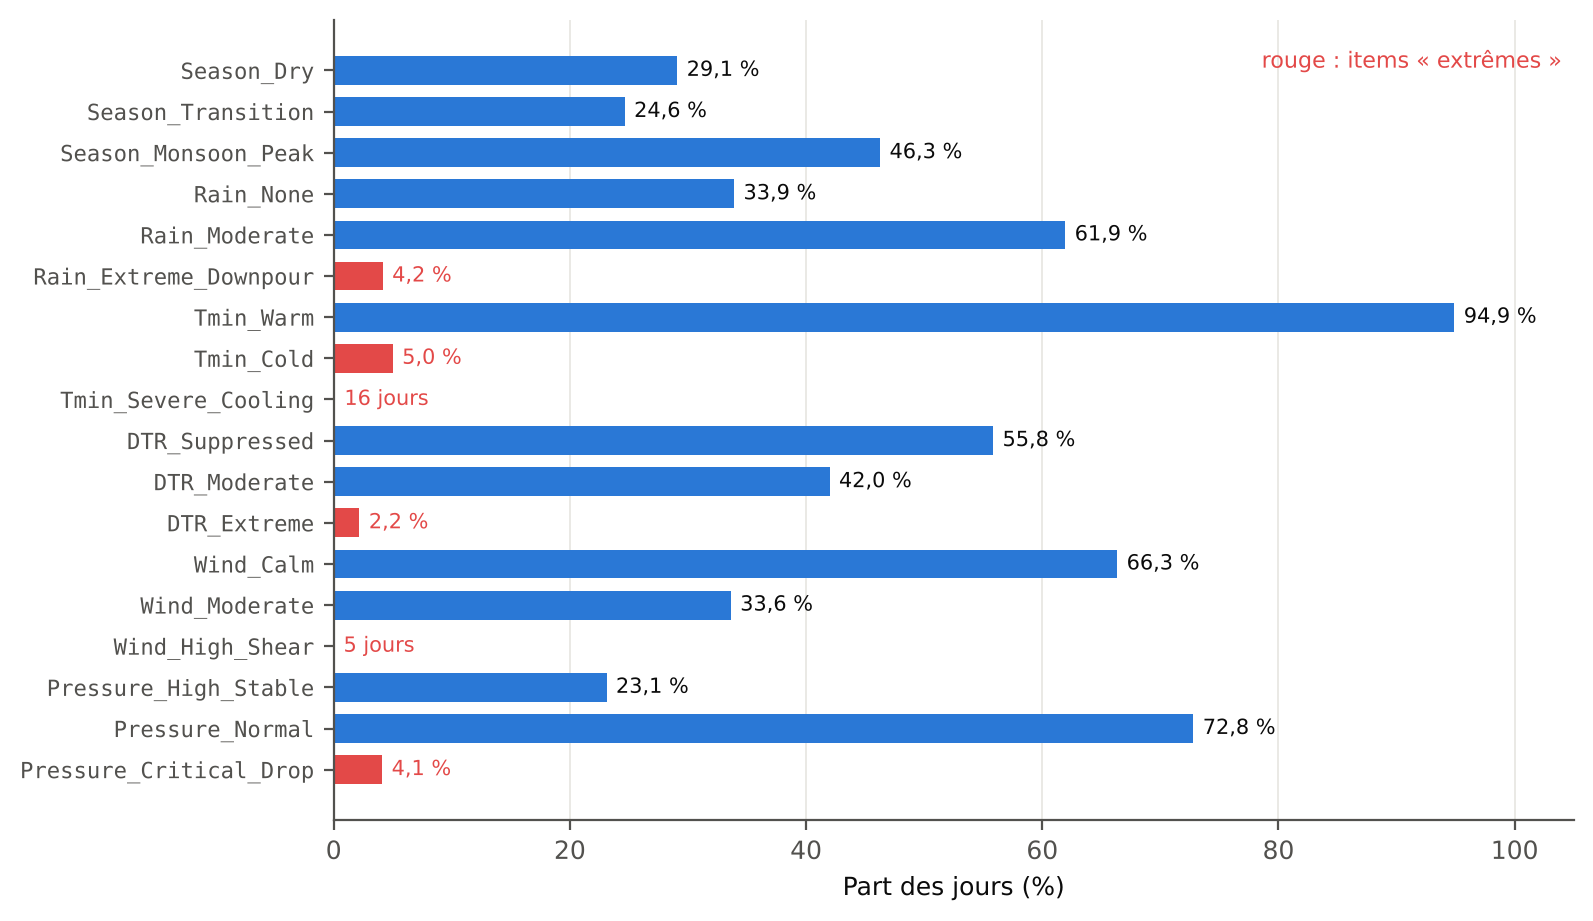
\includegraphics[width=0.85\linewidth]{figures/fig_items}
\caption{Part des jours portant chaque item. En rouge : les items « extrêmes » de l'énoncé.}
\label{fig:items}
\end{figure}

Cette répartition a trois conséquences pour l'extraction :
\begin{itemize}
  \item les items extrêmes sont rares (de 5 à 637 jours) : par anti-monotonie, aucun motif qui
        les contient ne peut dépasser leur propre support (au plus 4,2~\%) ;
  \item \itm{Tmin\_Severe\_Cooling} (\nTminSevereCooling~jours) et \itm{Wind\_High\_Shear}
        (\nWindHighShear~jours) sont presque vides et ne pourront apparaître dans aucune règle ;
  \item \itm{Tmin\_Warm} (\pTminWarm~\%) est omniprésent, ce qui justifie la métrique d'écart
        présentée en section~\ref{sec:metriques}.
\end{itemize}

Le tableau~\ref{tab:extremes_saisons} donne, pour chaque item extrême, la saison où il
survient. Il annonce déjà un résultat important pour H1 : \textbf{chaque extrême a sa propre
saison}.

\begin{table}[H]
\centering
\caption{Répartition saisonnière des jours portant chaque item extrême.}
\label{tab:extremes_saisons}
\tabin{tab_extremes_saisons}
\end{table}

\subsection{Encodage et passage à Weka}
\label{sec:weka}

Les transactions sont encodées en \textbf{18 attributs binaires} \{0, 1\}, un par item. Le
code vérifie que chaque ligne contient exactement six 1. Le tableau est exporté au format
ARFF, le format natif de Weka :

\begin{code}
\begin{verbatim}
@relation monoun_transactions

@attribute Season_Dry {0,1}
@attribute Season_Transition {0,1}
...
@attribute Pressure_Critical_Drop {0,1}

@data
1,0,0,1,0,0,0,1,0,0,1,0,0,1,0,0,1,0     <- 01/01/1983
\end{verbatim}
\end{code}

Pourquoi un encodage binaire plutôt que 6 attributs nominaux à 3 valeurs ? Le FP-Growth de Weka
n'accepte que des attributs binaires. Avec l'option \texttt{positiveIndex = 2}, seule la valeur
\texttt{1} est traitée comme un item : l'absence d'un item n'est jamais elle-même un item, ce
qui est exactement la logique « panier » du cours.

\paragraph{FP-Growth ou Apriori ?} Le cours détaille Apriori (« générer-et-élaguer »).
L'énoncé impose FP-Growth (« diviser-pour-régner »). Pour les mêmes minSupp et minConf, les deux
algorithmes produisent \textbf{exactement les mêmes motifs fréquents et les mêmes règles} ; seul
le coût de calcul diffère, FP-Growth évitant de générer des candidats. Nous avons donc suivi
l'énoncé.

\subsection{Configuration de Weka et justification}
\label{sec:config}

\begin{table}[H]
\centering
\caption{Paramètres de FP-Growth dans Weka et justification.}
\label{tab:config}
\footnotesize
\rowcolors{2}{GrisL}{white}
\begin{tabular}{>{\raggedright\arraybackslash}p{4.6cm}>{\raggedright\arraybackslash}p{2.1cm}p{7.5cm}}
\toprule
\rowcolor{NuitBleue!90}
\color{white}\textbf{Paramètre} & \color{white}\textbf{Valeur} & \color{white}\textbf{Pourquoi} \\
\midrule
\texttt{positiveIndex} & 2 & La 2\textsuperscript{e} valeur de \{0,1\}, soit 1, signifie « item présent ». \\
\texttt{metricType} & Confidence & Critère de fiabilité du cours. \\
\texttt{minMetric} & 0,7 & minConf : valeur utilisée dans l'exemple du cours. \\
\texttt{lowerBoundMinSupport} & 0,10 ; 0,05 ; 0,01 & minSupp : trois essais (voir ci-dessous). \\
\texttt{findAllRules}\newline\texttt{ForSupportLevel} & True & Sans cette option, Weka part d'un support de 100~\% et s'arrête dès qu'il a 10 règles : on n'obtiendrait que les règles les plus banales. \\
\texttt{maxNumberOfItems} & $-1$ & Pas de limite de taille des motifs (6 items au plus par jour). \\
\bottomrule
\end{tabular}
\end{table}

\paragraph{Pourquoi trois niveaux de minSupp ?} Le choix de minSupp découle de
l'anti-monotonie. Un item extrême couvre au plus 4,2~\% des jours : avec minSupp = 0,10 ou
0,05, \textbf{aucune règle ne peut le contenir}. Nous avons donc lancé :
\begin{itemize}
  \item 0,10 (au moins 1\,535 jours) : la structure générale du climat ;
  \item 0,05 (au moins 768 jours) : un niveau intermédiaire, pour vérifier la stabilité ;
  \item 0,01 (au moins 154 jours, soit environ 4 jours par an) : le seul niveau où les items
        extrêmes peuvent apparaître. C'est l'essai qui répond aux hypothèses.
\end{itemize}

Commande Weka de l'essai principal (enregistrée en tête de chaque fichier de résultats) :
\begin{code}[fontupper=\scriptsize\ttfamily]
\begin{verbatim}
weka.associations.FPGrowth -P 2 -I -1 -N 10 -T 0 -C 0.7 -D 0.05 -U 1.0 -M 0.01 -S
\end{verbatim}
\end{code}

\subsection{Post-traitement des règles}
\label{sec:post}

Les fichiers de résultats de Weka sont relus par une fonction Python qui extrait, pour chaque
règle, la prémisse, le conséquent, $n(X)$, $n(X \cup Y)$ et la confiance. On recalcule ensuite
le support du conséquent sur les transactions, puis on applique les deux filtres de la
section~\ref{sec:metriques} : règles informatives, puis non redondantes. La
figure~\ref{fig:nuage} montre que les règles non informatives ne se distinguent pas par leur
confiance : seule la comparaison avec $\operatorname{supp}(Y)$ permet de les repérer.

\begin{figure}[H]
\centering
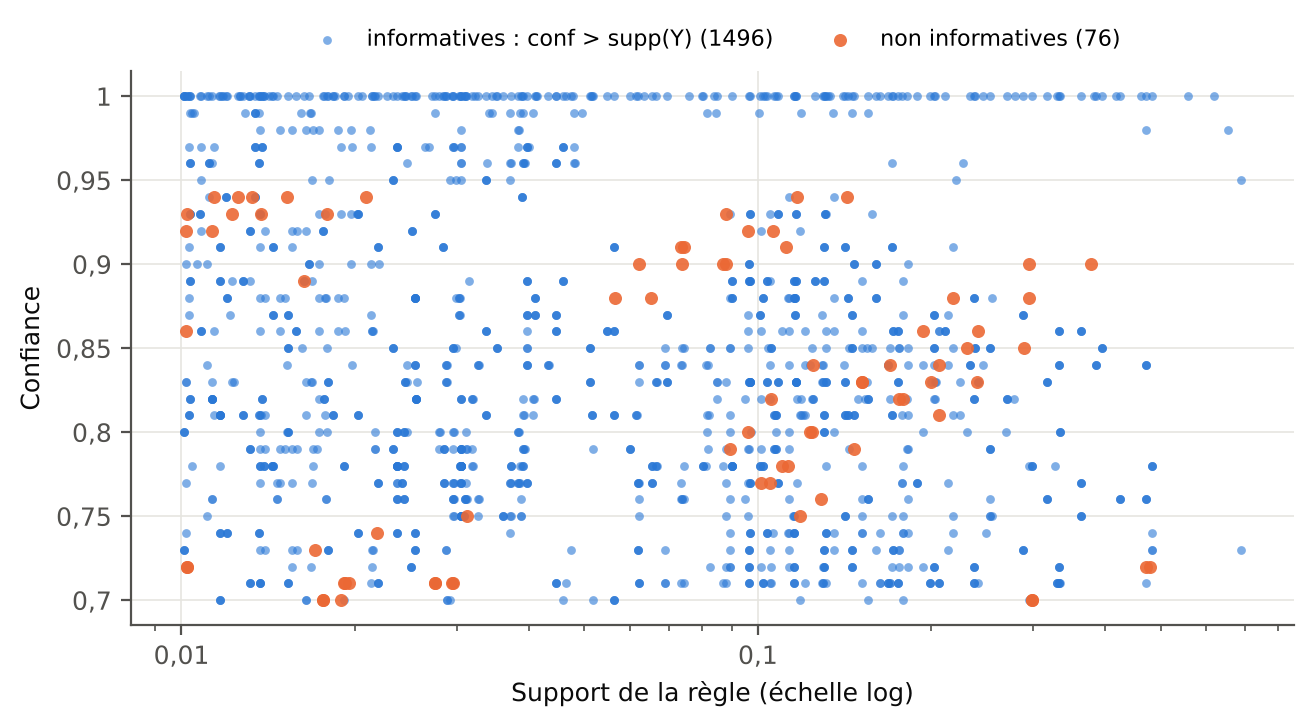
\includegraphics[width=0.82\linewidth]{figures/fig_nuage_regles}
\caption{Support et confiance des \NreglesBrutes{} règles de l'essai à minSupp = 0,01.}
\label{fig:nuage}
\end{figure}

\subsection{Analyse temporelle}
\label{sec:methode_temps}

L'éruption a eu lieu dans la nuit du 15 au 16 août 1984 (DOY 228). Nous avons retenu une
\textbf{fenêtre de 7 jours} se terminant le jour de l'éruption (DOY 222 à 228) : assez courte
pour décrire les conditions immédiates, assez longue pour ne pas dépendre d'un seul jour. La
\textbf{signature} est le motif présent tous ces jours-là. Sa réapparition est mesurée par le
nombre de jours par an qui la contiennent, de 1983 à 2024. Les fenêtres de 3, 14 et 30 jours
servent de test de robustesse.

\needspace{12\baselineskip}
%═══════════════════════════════════════════════════════════════════════
\section{Résultats et interprétation}
\label{sec:resultats}
%═══════════════════════════════════════════════════════════════════════

\subsection{Vue d'ensemble des trois essais}

\begin{table}[H]
\centering
\caption{Nombre de règles par essai (minConf = 0,7).}
\label{tab:essais}
\tabin{tab_essais}
\end{table}

\begin{itemize}
  \item Les filtres retirent environ \textbf{trois règles sur quatre} : à minSupp = 0,01, on
        passe de \NreglesBrutes{} à \NreglesInf{} règles informatives, puis à
        \NreglesClean{} règles non redondantes. \NreglesNonInf{} règles dépassent minConf tout
        en étant non informatives, et \NreglesTminWarm{} ont pour seul conséquent
        \itm{Tmin\_Warm}.
  \item Comme prévu par l'anti-monotonie, \textbf{aucune règle des essais à 0,10 et 0,05 ne
        contient d'item extrême}. Elles décrivent uniquement la météo ordinaire.
\end{itemize}

\subsection{Les règles de la météo ordinaire}

\begin{table}[H]
\centering
\caption{Règles les plus marquées sans item extrême (essai à 0,01, règles filtrées).}
\label{tab:ordinaires}
\tabin{tab_regles_ordinaires}
\end{table}

Les règles les plus fortes décrivent la \textbf{saison sèche} : un vent modéré, une pression
haute et une amplitude thermique modérée annoncent presque à coup sûr un jour sans pluie
(confiance de 0,94 à 0,98, contre 34~\% de jours secs en moyenne), et ces conditions
désignent la saison sèche avec une confiance de 0,92. Ces règles, physiquement cohérentes
(air sec, ciel dégagé, pression haute), confirment que la discrétisation capte bien la
structure du climat.

\subsection{Les règles impliquant les items extrêmes}
\label{sec:res_extremes}

À minSupp = 0,01, quatre items extrêmes apparaissent dans les règles filtrées :
\itm{Tmin\_Cold} (\nrTminCold{} règles), \itm{Rain\_Extreme\_Downpour}
(\nrRainExtremeDownpour), \itm{Pressure\_Critical\_Drop} (\nrPressureCriticalDrop) et
\itm{DTR\_Extreme} (\nrDTRExtreme). Les tableaux suivants donnent les plus marquées.

\begin{table}[H]
\centering
\caption{Règles avec \itm{Rain\_Extreme\_Downpour} (pluie $> 20$ mm).}
\label{tab:r_rain}
\tabin{tab_regles_Rain_Extreme_Downpour}
\end{table}

\textbf{Lecture.} Une pluie extrême accompagnée d'un vent modéré tombe dans 94~\% des cas en pic
de mousson sous un ciel couvert (DTR faible), contre 39~\% des jours en moyenne. Les pluies
extrêmes sont des \textbf{pluies de mousson}, par nuits douces : elles ne s'accompagnent pas de
refroidissement nocturne.

\begin{table}[H]
\centering
\caption{Règles avec \itm{Pressure\_Critical\_Drop} (pression $< 88{,}4$ kPa).}
\label{tab:r_pression}
\tabin{tab_regles_Pressure_Critical_Drop}
\end{table}

\textbf{Lecture.} Une chute de pression critique avec une pluie modérée survient dans 83 à 87~\%
des cas en \textbf{saison de transition} (mars à mai), contre 25~\% des jours en moyenne. C'est
cohérent avec le cycle de la figure~\ref{fig:climatologie} : la pression est au plus bas en mars.

\begin{table}[H]
\centering
\caption{Règles avec \itm{Tmin\_Cold} (température minimale entre 11 et 14 °C).}
\label{tab:r_froid}
\tabin{tab_regles_Tmin_Cold}
\end{table}

\textbf{Lecture.} Les nuits froides tombent presque toutes un jour sec de \textbf{saison sèche}
(confiance de 0,97 à 1,00, contre 26 à 29~\% des jours). Le refroidissement nocturne est un
phénomène de ciel dégagé, pas de mousson.

\begin{table}[H]
\centering
\caption{Règles avec \itm{DTR\_Extreme} (amplitude thermique $> 14$ °C).}
\label{tab:r_dtr}
\tabin{tab_regles_DTR_Extreme}
\end{table}

\textbf{Lecture.} Les très fortes amplitudes thermiques vont avec un temps sec et venté
(confiance jusqu'à 0,92, contre 19~\% des jours) : c'est aussi un phénomène de saison sèche.

\begin{reponse}[Ce que disent ces règles]
Chaque facteur de risque de l'énoncé est attaché à une \textbf{saison différente} : la pluie
extrême à la mousson, la chute de pression à la transition, le refroidissement et la forte
amplitude thermique à la saison sèche. \textbf{Aucune des \NreglesBrutes{} règles ne contient
deux items extrêmes.}
\end{reponse}

\subsection{Les combinaisons composites de l'énoncé}
\label{sec:res_composites}

L'absence de règle reliant deux extrêmes pourrait venir du seuil minSupp. Nous avons donc
compté directement les jours où ils coïncident, sans seuil (tableau~\ref{tab:composites}).

\begin{table}[H]
\centering
\caption{Nombre de jours réunissant plusieurs facteurs de risque (1983--2024).}
\label{tab:composites}
\tabin{tab_composites}
\end{table}

Aucune paire ne dépasse 16 jours en 42 ans, très loin des 154 jours exigés par minSupp = 0,01.
La combinaison décrite par l'énoncé (chute de pression, pluie extrême et nuit froide) ne
s'observe \textbf{aucun jour}.

\subsection{La fenêtre pré-éruption et sa signature}
\label{sec:res_fenetre}

\begin{table}[H]
\centering
\caption{Les 7 jours précédant l'éruption (1984). Unités : mm, °C, °C, m/s, kPa. Tous les jours
sont aussi \itm{Season\_Monsoon\_Peak}, \itm{Rain\_Moderate}, \itm{Tmin\_Warm} et
\itm{Pressure\_Normal}.}
\label{tab:fenetre}
\tabin{tab_fenetre}
\end{table}

Aucun item extrême n'apparaît dans la fenêtre : pluie modérée, nuits douces, ciel plutôt
couvert, vent calme et pression normale. La signature commune aux 7 jours est :
\begin{formule}
\textbf{Signature} $= \{$\signature$\}$, \quad $\operatorname{supp} = \sigSupp$
\end{formule}

Son support de \sigSupp{} signifie qu'elle s'observe \textbf{environ un jour sur quatre} sur
toute la série. Les règles filtrées que ces 7 jours vérifient (tableau~\ref{tab:r_fenetre})
décrivent la mousson ordinaire. Seule la première apporte une information nette : en pic de
mousson, la pluie est le plus souvent modérée (85~\% contre 62~\%). Les autres ont un écart
presque nul.

\begin{table}[H]
\centering
\caption{Règles (essai à 0,01, filtrées) vérifiées par les 7 jours de la fenêtre.}
\label{tab:r_fenetre}
\tabin{tab_regles_fenetre}
\end{table}

\paragraph{Robustesse au choix de la fenêtre.} Le tableau~\ref{tab:sensibilite} refait
l'analyse avec des fenêtres de 3, 14 et 30 jours.

\begin{table}[H]
\centering
\caption{Sensibilité de la signature à la taille de la fenêtre. Extr. : nombre d'items extrêmes
dans la fenêtre ; 1984 : jours de 1984 portant la signature ; rang de 1984 parmi les 42 années
(* : ex æquo avec d'autres années) ; pente en jours par décennie.}
\label{tab:sensibilite}
\tabin{tab_sensibilite}
\end{table}

\begin{itemize}
  \item Quelle que soit la fenêtre, la signature est faite d'items \textbf{ordinaires}. Sur
        30 jours, un seul jour porte un item extrême : une pluie de plus de 20~mm le
        24 juillet, trois semaines avant l'éruption.
  \item Avec 3 jours, la signature contient les 6 items ordinaires de la mousson, et 1984 est
        l'année qui en compte le plus (80 jours) : la mousson 1984 a été particulièrement
        \emph{ordinaire} (vent calme, pluie modérée, ciel couvert), et non extrême.
  \item Plus la fenêtre est longue, plus la signature se réduit à « mousson et nuits douces »,
        ce qui décrit tous les jours de mousson.
\end{itemize}

\subsection{Réapparition de 1983 à 2024}
\label{sec:res_temps}

\paragraph{La signature.} La figure~\ref{fig:signature} donne le nombre de jours par an qui
présentent la signature des 7 jours.

\begin{figure}[H]
\centering
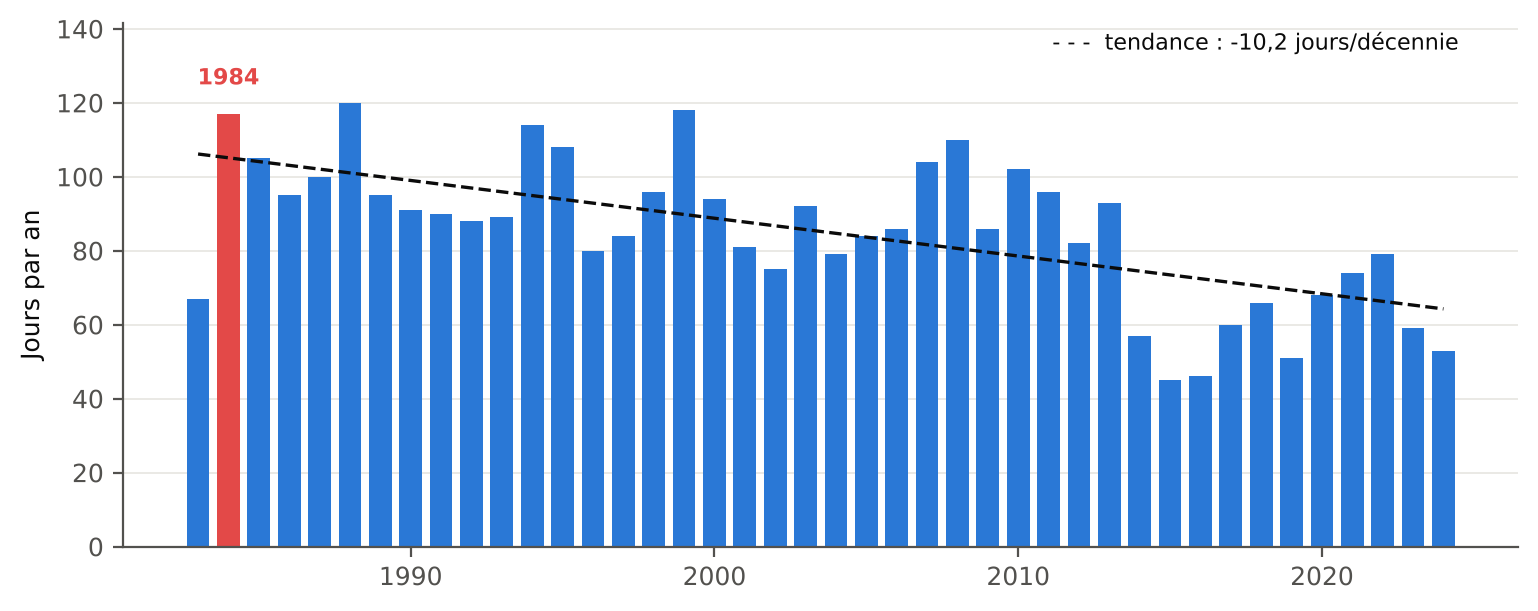
\includegraphics[width=0.95\linewidth]{figures/fig_signature_par_an}
\caption{Jours par an présentant la signature pré-éruption (1984 en rouge) et tendance linéaire.}
\label{fig:signature}
\end{figure}

\begin{itemize}
  \item La signature apparaît en moyenne \sigMoy~jours par an. L'année 1984 en compte
        \sigMilleNeuf{} et se classe \sigRang\textsuperscript{e} sur 42 : élevée, mais pas
        exceptionnelle.
  \item La signature \textbf{recule} : pente de \sigPente~jours par décennie, tendance
        significative (Mann-Kendall : $\tau = \sigTau$, $p < 0{,}001$).
  \item La baisse se concentre après 2013 : \sigAvant~jours par an en moyenne sur 1983--2013,
        contre \sigApres{} sur 2014--2024.
\end{itemize}

\paragraph{Pourquoi ce recul ?} Deux effets se combinent :
\begin{itemize}
  \item \textbf{la pression} : la moyenne de mousson passe de \psAvant~kPa (1983--2013) à
        \psApres~kPa (2014--2024), soit +\psDelta~kPa. Elle se place juste au niveau du seuil de
        88,7~kPa (figure~\ref{fig:pression}) : de nombreux jours basculent de
        \itm{Pressure\_Normal} à \itm{Pressure\_High\_Stable} et sortent de la signature ;
  \item \textbf{les pluies extrêmes de mousson} passent de \rexAvant{} à \rexApres~jours par
        an en moyenne. Ces jours remplacent \itm{Rain\_Moderate} et sortent eux aussi de la
        signature.
\end{itemize}

\begin{figure}[H]
\centering
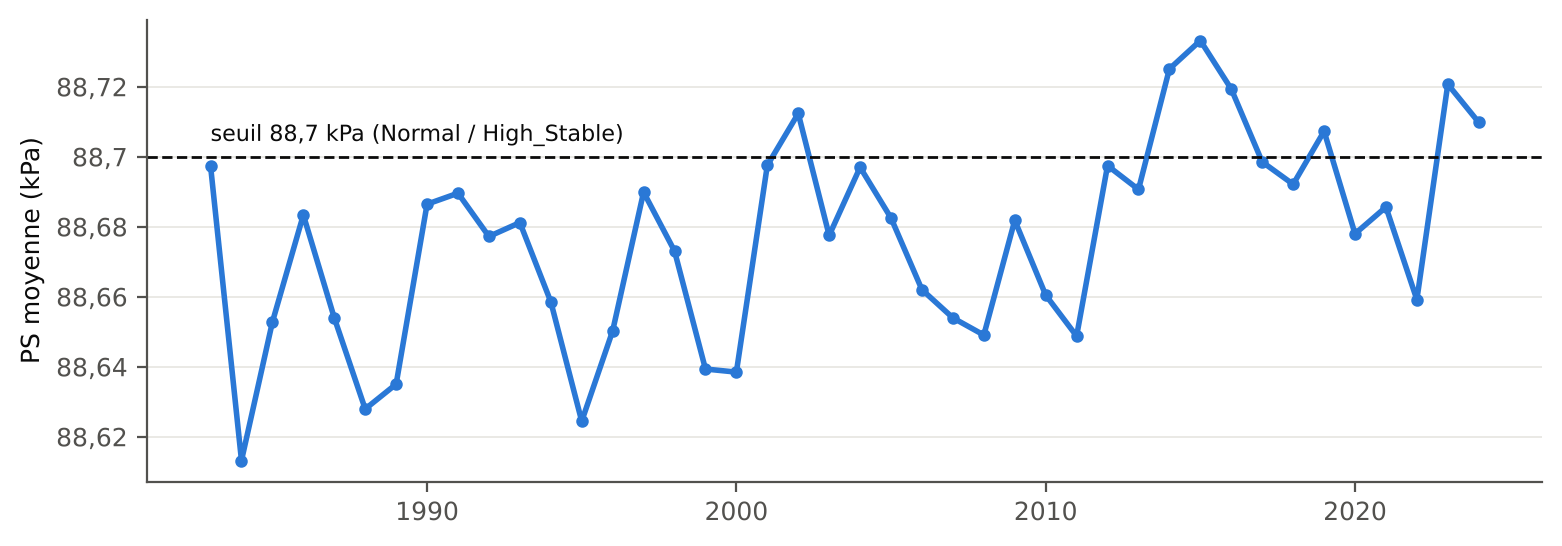
\includegraphics[width=0.95\linewidth]{figures/fig_pression_mousson}
\caption{Pression moyenne en pic de mousson (DOY 151--319) et seuil de 88,7~kPa.}
\label{fig:pression}
\end{figure}

\begin{remarque}
L'effet de pression est un décalage de quelques centièmes de kPa situé exactement sur un seuil.
Le comptage est donc sensible au choix de 88,7~kPa : il ne faut pas y lire un changement
climatique majeur. La hausse des pluies extrêmes en mousson est un signal plus net.
\end{remarque}

\paragraph{Les items extrêmes.} La figure~\ref{fig:extremes} et le
tableau~\ref{tab:tendances} donnent l'évolution de chaque item extrême.

\begin{figure}[H]
\centering
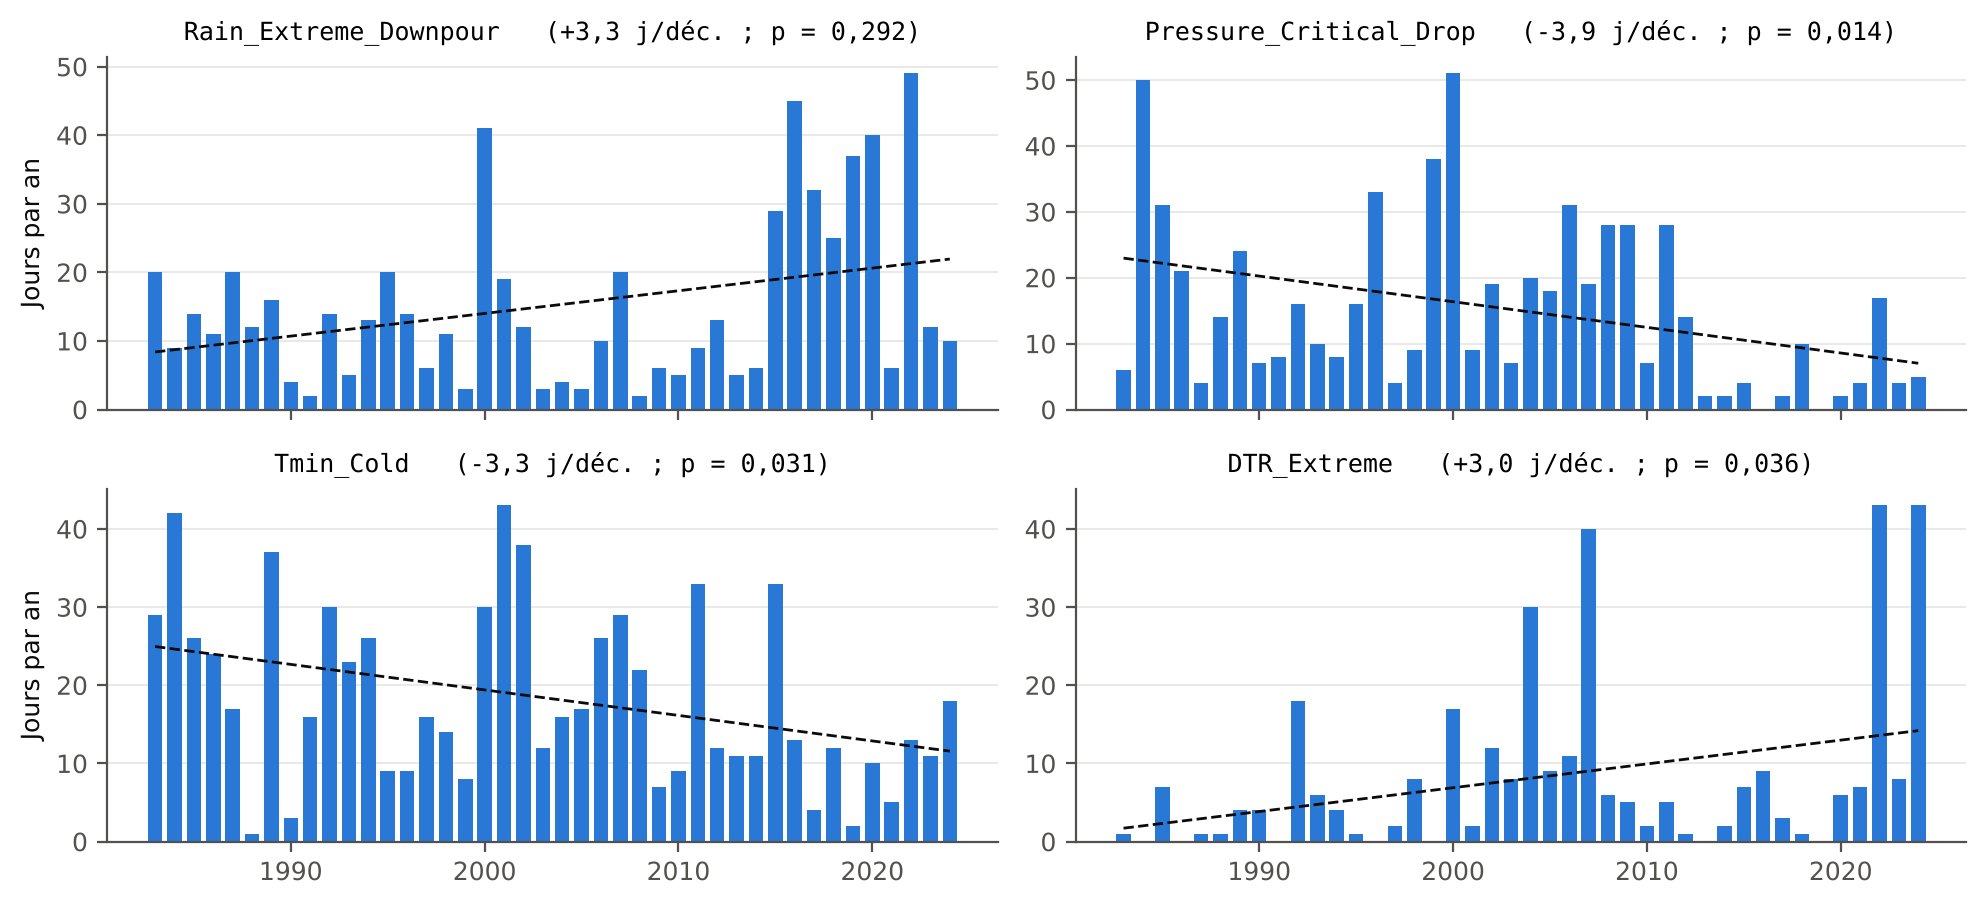
\includegraphics[width=\linewidth]{figures/fig_extremes_par_an}
\caption{Jours par an portant chaque item extrême, avec tendance linéaire et p-valeur de
Mann-Kendall.}
\label{fig:extremes}
\end{figure}

\begin{table}[H]
\centering
\caption{Tendances des items extrêmes sur 1983--2024.}
\label{tab:tendances}
\tabin{tab_tendances}
\end{table}

\begin{itemize}
  \item \textbf{Nuits froides} : en baisse (\penteTminCold~j/décennie, $p = \pvalTminCold$).
        C'est cohérent avec le réchauffement : la température minimale moyenne passe de
        \tminQuatreVingt~°C (1983--1989) à \tminVingt~°C (2020--2024).
  \item \textbf{Chutes de pression critiques} : en baisse (\pentePressureCriticalDrop~j/décennie,
        $p = \pvalPressureCriticalDrop$).
  \item \textbf{Fortes amplitudes thermiques} : en hausse (+\penteDTRExtreme~j/décennie,
        $p = \pvalDTRExtreme$).
  \item \textbf{Pluies extrêmes} : hausse non significative sur l'année entière
        ($p = \pvalRainExtremeDownpour$), malgré la nette hausse en mousson depuis 2014.
\end{itemize}

\needspace{12\baselineskip}
%═══════════════════════════════════════════════════════════════════════
\section{Validation des hypothèses}
\label{sec:verdict}
%═══════════════════════════════════════════════════════════════════════

\begin{hypothese}{H0 — Des seuils climatologiques : partiellement rejetée}
\textbf{Ce qui la soutient :} le seuil de pluie extrême (20~mm) est proche du $P_{95}$ réel
(\PnfRain~mm) ; 4,2~\% des jours sont extrêmes, proche des 5~\% attendus.

\textbf{Ce qui la contredit :} le $P_{10}$ réel de la température minimale est de
\PdixTmin~°C et non 11~°C ; \itm{Tmin\_Severe\_Cooling} ne couvre que 0,1~\% des jours et
\itm{Wind\_High\_Shear} 5 jours en 42 ans.

\textbf{Conséquence :} deux des facteurs de risque de l'énoncé (refroidissement sévère, vent
fort) sont \emph{inobservables} par les règles d'association avec ces seuils. Nous les avons
gardés pour respecter la consigne, mais cette limite pèse sur toutes les conclusions.
\end{hypothese}

\begin{hypothese}{H1 — Les extrêmes se combinent : rejetée}
\textbf{Pourquoi :} aucune des \NreglesBrutes{} règles ne contient deux items extrêmes ; chaque
extrême est associé à une saison différente (tableaux~\ref{tab:extremes_saisons}
à~\ref{tab:r_dtr}) ; les coïncidences comptées sans seuil sont quasi nulles, et la combinaison
de l'énoncé n'apparaît aucun jour (tableau~\ref{tab:composites}). Les extrêmes météo du lac
Monoun sont des phénomènes \emph{saisonniers et séparés}, pas des événements composites.
\end{hypothese}

\begin{hypothese}{H2 — Une signature extrême a précédé l'éruption : rejetée}
\textbf{Pourquoi :} aucun item extrême dans les 7 jours qui précèdent l'éruption, ni dans les
fenêtres de 3 et 14 jours, et un seul jour de pluie forte sur 30 jours. La signature,
$\{$\signature$\}$, est un motif fréquent (support \sigSupp) de la mousson ordinaire, et 1984
n'est pas une année exceptionnelle pour ce motif (\sigRang\textsuperscript{e} sur 42).
\end{hypothese}

\begin{hypothese}{H3 — Réapparition croissante : rejetée}
\textbf{Pourquoi :} la signature recule de \sigPenteAbs~jours par décennie environ, de façon
significative. Les extrêmes ne montrent pas de hausse d'ensemble : les nuits froides et les
chutes de pression diminuent, seules les fortes amplitudes thermiques augmentent, et les pluies
extrêmes n'augmentent significativement qu'en mousson depuis 2014. Le réchauffement est bien
visible (nuits plus chaudes), mais il \emph{réduit} le refroidissement nocturne que l'énoncé
présentait comme moteur de l'inversion.
\end{hypothese}

\begin{table}[H]
\centering
\caption{Synthèse des verdicts.}
\label{tab:verdicts}
\small
\rowcolors{2}{GrisL}{white}
\begin{tabular}{p{1cm}>{\raggedright\arraybackslash}p{6.3cm}>{\raggedright\arraybackslash}p{2.6cm}>{\raggedright\arraybackslash}p{4.1cm}}
\toprule
\rowcolor{NuitBleue!90}
\color{white}\textbf{Hyp.} & \color{white}\textbf{Énoncé} & \color{white}\textbf{Verdict} & \color{white}\textbf{Preuve principale} \\
\midrule
H0 & Les seuils sont des centiles climatologiques & Partiellement rejetée & $P_{10}$ de Tmin = \PdixTmin~°C \\
H1 & Les extrêmes se combinent & \textcolor{RougeL}{\textbf{Rejetée}} & 0 règle à deux extrêmes \\
H2 & Signature extrême avant l'éruption & \textcolor{RougeL}{\textbf{Rejetée}} & 0 item extrême sur 7 jours \\
H3 & Réapparition croissante & \textcolor{RougeL}{\textbf{Rejetée}} & Pente \sigPente~j/déc. \\
\bottomrule
\end{tabular}
\end{table}

\needspace{12\baselineskip}
%═══════════════════════════════════════════════════════════════════════
\section{Discussion et limites}
%═══════════════════════════════════════════════════════════════════════

\paragraph{Un résultat cohérent avec la littérature.} Les règles d'association ne trouvent pas
de déclencheur météorologique. Ce résultat rejoint l'explication retenue par Sigurdsson et al.
(1987) : la stratification du lac aurait été rompue par un \textbf{séisme suivi d'un glissement
de terrain sous-lacustre} survenus le 15 août 1984, autrement dit par un déclencheur interne au
lac, invisible dans des données météorologiques. Notre analyse ne prouve pas cette explication,
mais elle écarte la piste météorologique telle que l'énoncé la formule.

\paragraph{Limites.}
\begin{itemize}
  \item \textbf{Un seul événement.} La signature repose sur un unique épisode : on ne peut pas
        valider statistiquement une « signature de risque » avec un seul cas.
  \item \textbf{Données de réanalyse.} MERRA-2 fournit des moyennes sur une maille d'environ
        50~km, qui lissent les extrêmes locaux (orage isolé, rafale, refroidissement de la
        surface du lac lui-même).
  \item \textbf{Seuils fixes.} Plusieurs seuils ne correspondent pas aux centiles annoncés, et le
        seuil de pression de 88,7~kPa tombe sur la moyenne de mousson, ce qui rend certains
        comptages sensibles (H0).
  \item \textbf{Co-occurrence et causalité.} Une règle d'association exprime une co-occurrence,
        jamais une relation de cause à effet.
  \item \textbf{Tests de tendance.} Le test de Mann-Kendall suppose des années indépendantes ; une
        éventuelle autocorrélation n'est pas prise en compte.
  \item \textbf{Réapparition et risque.} Le lac Monoun est dégazé artificiellement depuis le
        début des années 2000 : une configuration météo qui réapparaît ne représente plus le
        même risque qu'en 1984.
\end{itemize}

\needspace{12\baselineskip}
%═══════════════════════════════════════════════════════════════════════
\section{Conclusion}
%═══════════════════════════════════════════════════════════════════════

Nous avons transformé 42 ans de données météorologiques journalières en une base de
\Njours~transactions de 6 items, puis extrait les règles d'association avec FP-Growth dans
Weka, en jugeant les règles par le support, la confiance et l'écart entre la confiance et la
fréquence habituelle du conséquent.

Les résultats répondent à la question centrale :
\begin{itemize}
  \item \textbf{les extrêmes ne se combinent pas} : pluies extrêmes en mousson, chutes de
        pression en transition, nuits froides en saison sèche ;
  \item \textbf{les jours qui précèdent l'éruption sont ordinaires} : leur signature,
        $\{$\signature$\}$, décrit environ un jour sur quatre ;
  \item \textbf{cette signature recule} d'environ \sigPenteAbs~jours par décennie, et le
        réchauffement réduit les nuits froides au lieu de multiplier les conditions de risque.
\end{itemize}

Les quatre hypothèses issues de l'énoncé sont rejetées ou partiellement rejetées. La
catastrophe de 1984 ne semble pas avoir été précédée d'une configuration météorologique
particulière, ce qui est cohérent avec un déclencheur géologique.

\paragraph{Perspectives.} Trois prolongements renforceraient l'étude : refaire l'analyse avec
des seuils fixés par les centiles réels de la série ; appliquer la même démarche au lac Nyos
(21 août 1986) pour disposer d'un second événement ; utiliser des données de station ou de
plus haute résolution, moins lissées que la réanalyse.

\newpage
%═══════════════════════════════════════════════════════════════════════
\section*{Références}
\addcontentsline{toc}{section}{Références}
%═══════════════════════════════════════════════════════════════════════

\begin{itemize}[label={},leftmargin=1em,itemsep=4pt]
\small
  \item Agrawal, R., Imieliński, T. et Swami, A. (1993). Mining association rules between sets
        of items in large databases. \emph{Proceedings of the ACM SIGMOD International
        Conference on Management of Data}, 207--216.
  \item Han, J., Pei, J. et Yin, Y. (2000). Mining frequent patterns without candidate
        generation. \emph{Proceedings of the ACM SIGMOD International Conference on Management
        of Data}, 1--12.
  \item Sigurdsson, H., Devine, J. D., Tchoua, F. M. et al. (1987). Origin of the lethal gas
        burst from Lake Monoun, Cameroun. \emph{Journal of Volcanology and Geothermal Research},
        31(1--2). doi:10.1016/0377-0273(87)90002-3.
  \item ETCCDI — Expert Team on Climate Change Detection and Indices. \emph{Definitions of the 27
        core indices}. \url{https://etccdi.pacificclimate.org/list_27_indices.shtml}.
  \item NASA POWER — Prediction Of Worldwide Energy Resources, données journalières MERRA-2.
        \url{https://power.larc.nasa.gov}.
  \item Witten, I. H., Frank, E., Hall, M. A. et Pal, C. J. (2016). \emph{Data Mining: Practical
        Machine Learning Tools and Techniques} (4\textsuperscript{e} éd.). Morgan Kaufmann.
  \item Support de cours : \emph{Fouille de données — Règles d'association}, Master 2 Data
        Science, ENSPY, 2026--2027.
\end{itemize}

\newpage
%═══════════════════════════════════════════════════════════════════════
\section*{Annexe — Reproductibilité}
\addcontentsline{toc}{section}{Annexe — Reproductibilité}
%═══════════════════════════════════════════════════════════════════════

Le code, les données et les résultats sont disponibles sur
\url{https://github.com/mentalist011101/monoun-limnic-eruption-mining}.

\begin{code}
\begin{verbatim}
data/raw/          donnees brutes NASA POWER
data/processed/    transactions (.csv, .arff), index.csv
src/               preparation.py (phase 1), analyse.py (phase 3)
notebooks/         01_preparation.ipynb, 02_analyse.ipynb
weka/results/      sorties FP-Growth (minSupp 0,10 / 0,05 / 0,01)
reports/latex/     ce rapport : main.tex, generate_assets.py
\end{verbatim}
\end{code}

\noindent Ordre d'exécution :
\begin{enumerate}
  \item \texttt{notebooks/01\_preparation.ipynb} ;
  \item FP-Growth dans Weka sur \texttt{transactions\_binary.arff}, avec les paramètres du
        tableau~\ref{tab:config} ;
  \item \texttt{notebooks/02\_analyse.ipynb} ;
  \item \texttt{reports/latex/generate\_assets.py}, puis compilation de \texttt{main.tex}.
\end{enumerate}

\end{document}
